%==============================================================================
%  FertiLuna: a privacy-preserving, on-device machine-learning system for
%  menstrual-cycle analysis.
%
%  Authors:
%    Bijou Kachungunu <bijoukach2000@gmail.com>
%    Gabriel Mougard <gabriel.mougard@gmail.com>
%
%  Build:  latexmk -pdf main.tex   (biber for bibliography)
%  Figures are PlantUML diagrams rendered to SVG then converted to PDF
%  (see build.sh / the puml/ and figures/ directories).
%==============================================================================
\documentclass[11pt,a4paper]{article}

%------------------------------ Fonts & encoding ------------------------------
\usepackage[T1]{fontenc}
\usepackage[utf8]{inputenc}
% Text font now; the matching math font (newtxmath) is loaded AFTER amsmath /
% amsthm below so that newtxmath can patch the AMS symbol clashes correctly.
\usepackage{newtxtext}
\usepackage{microtype}

%------------------------------ Math ------------------------------------------
% Order matters: amsmath / amsthm, THEN newtxmath. newtxmath supplies the
% amssymb (blackboard, etc.) glyphs, so amssymb is not loaded separately to
% avoid the \Bbbk / \openbox redefinition clashes.
\usepackage{amsmath,amsthm}
\usepackage{newtxmath}
\usepackage{mathtools}
\usepackage{bm}
\usepackage{sourcecodepro}  % monospaced font for code/inline \texttt

%------------------------------ Layout ----------------------------------------
\usepackage[a4paper,margin=1in]{geometry}
\usepackage{titlesec}
\usepackage{enumitem}
\setlist{itemsep=2pt,topsep=3pt}
\usepackage{fancyhdr}
\usepackage{abstract}

%------------------------------ Graphics & tables -----------------------------
\usepackage{graphicx}
\usepackage{float}
\usepackage{booktabs}
\usepackage{multirow}
\usepackage{makecell}
\usepackage{colortbl}
\usepackage{caption}
\usepackage{subcaption}
\usepackage[table]{xcolor}
\usepackage{siunitx}
\usepackage{pgfplots}
\pgfplotsset{compat=1.18}
\usepackage{adjustbox}
\usepackage{pdflscape}

%------------------------------ Code listings ---------------------------------
\usepackage{listings}

%------------------------------ Hyperlinks ------------------------------------
\usepackage[colorlinks=true,linkcolor=NavyBlue,citecolor=ForestGreen,
            urlcolor=NavyBlue,breaklinks=true]{hyperref}
\usepackage{url}

%------------------------------ Bibliography ----------------------------------
\usepackage[backend=biber,style=numeric,sorting=none,maxbibnames=6]{biblatex}
\addbibresource{references.bib}

%------------------------------ Colours ---------------------------------------
\definecolor{NavyBlue}{RGB}{21,101,192}
\definecolor{ForestGreen}{RGB}{46,125,50}
\definecolor{CodeBg}{RGB}{246,248,250}
\definecolor{CodeKw}{RGB}{167,29,93}
\definecolor{CodeStr}{RGB}{3,47,98}
\definecolor{CodeCom}{RGB}{106,115,125}
\definecolor{RuleGray}{RGB}{120,144,156}

%------------------------------ Listing styles --------------------------------
\lstdefinestyle{mono}{
  basicstyle=\ttfamily\footnotesize,
  backgroundcolor=\color{CodeBg},
  keywordstyle=\color{CodeKw}\bfseries,
  stringstyle=\color{CodeStr},
  commentstyle=\color{CodeCom}\itshape,
  numberstyle=\tiny\color{RuleGray},
  numbers=left,numbersep=8pt,
  frame=single,rulecolor=\color{RuleGray!50},
  framexleftmargin=4pt,xleftmargin=14pt,
  breaklines=true,showstringspaces=false,
  columns=fullflexible,keepspaces=true,
  tabsize=2,captionpos=b,
}
\lstset{style=mono}
\lstdefinelanguage{ts}{
  morekeywords={const,let,async,await,function,return,new,interface,type,import,
                from,export,for,if,else,throw,class,extends,this,null,number},
  morecomment=[l]{//},morecomment=[s]{/*}{*/},morestring=[b]",morestring=[b]'
}

%------------------------------ Theorem-like envs -----------------------------
\newtheorem{definition}{Definition}
\newtheorem{property}{Property}

%------------------------------ Section format --------------------------------
\titleformat{\section}{\large\bfseries\color{NavyBlue!85!black}}{\thesection}{0.6em}{}
\titleformat{\subsection}{\normalsize\bfseries\color{black}}{\thesubsection}{0.6em}{}

%------------------------------ Header ----------------------------------------
\pagestyle{fancy}
\fancyhf{}
\fancyhead[L]{\footnotesize\itshape FertiLuna: On-Device ML for Cycle Analysis}
\fancyhead[R]{\footnotesize\thepage}
\renewcommand{\headrulewidth}{0.4pt}

%------------------------------ Macros ----------------------------------------
\newcommand{\code}[1]{\texttt{\small #1}}
\newcommand{\file}[1]{\texttt{\small\color{NavyBlue!70!black}#1}}
\DeclareMathOperator*{\softmax}{softmax}
\DeclareMathOperator*{\argmax}{arg\,max}

%==============================================================================
\begin{document}

%------------------------------ Title -----------------------------------------
\begin{titlepage}
\centering
\vspace*{1.5cm}
{\color{RuleGray}\rule{\textwidth}{0.8pt}}\\[0.6cm]
{\LARGE\bfseries FertiLuna: a privacy-preserving, on-device\\[0.25cm]
machine-learning system for\\[0.25cm] menstrual-cycle analysis\par}
\vspace{0.5cm}
{\large A dual-model (vision $+$ forest) architecture\\
shipped entirely to the web browser\par}
\vspace{0.4cm}
{\color{RuleGray}\rule{\textwidth}{0.8pt}}\\[1.2cm]

\begin{minipage}[t]{0.48\textwidth}
\raggedright
{\large\textbf{Bijou Kachungunu}}\\[0.2cm]
{\normalsize \href{mailto:bijoukach2000@gmail.com}{bijoukach2000@gmail.com}}
\end{minipage}\hfill
\begin{minipage}[t]{0.48\textwidth}
\raggedleft
{\large\textbf{Gabriel Mougard}}\\[0.2cm]
{\normalsize \href{mailto:gabriel.mougard@gmail.com}{gabriel.mougard@gmail.com}}
\end{minipage}\\[1.6cm]

\begin{minipage}{0.85\textwidth}
\small\itshape
\centering
We describe the design, training, and deployment of FertiLuna, a fertility-data
analysis tool whose entire machine-learning stack runs inside the user's web
browser. Two complementary model families work together: a depthwise-separable
\emph{convolutional vision network} that digitizes chart screenshots, and a
calibrated \emph{random-forest classifier} paired with an isolation forest for
out-of-distribution detection. Both are trained on physiologically grounded
synthetic data, exported to ONNX, and served as same-origin static assets that
are cached and version-controlled in the browser. No account is created, and no
cycle datum ever leaves the device.
\end{minipage}

\vfill
{\normalsize Technical report \textbullet{} \today}\\
{\footnotesize\color{RuleGray} Source, PlantUML diagrams, and figures accompany this document.}
\end{titlepage}

%------------------------------ Abstract --------------------------------------
\begin{abstract}
\noindent
Health applications that handle reproductive data sit at an awkward crossroads:
machine learning offers real analytical value, but the underlying records are
intimately personal. FertiLuna resolves that tension by moving \emph{all}
inference to the client. Models are downloaded once, validated against a
cryptographic checksum, cached in IndexedDB, and executed with ONNX Runtime Web
compiled to WebAssembly. The system combines two stages with complementary
inductive biases. The \emph{vision} stage is a deterministic classical
computer-vision pipeline (OpenCV-style segmentation, multi-axis OCR with RANSAC
line fitting, and geometric marker detection), aided by a small PaddleOCR text
recognizer. It reads a screenshot of a fertility-app chart and recovers per-day
basal-body-temperature (BBT) and luteinizing-hormone (LH) values, together with
the chart's temperature unit and its calendar table, removing the need for
manual transcription. We also built a convolutional-network alternative that we
deliberately did not ship, and we explain why the deterministic pipeline was
preferred. The \emph{forest} stage is a single prefit random forest with Platt
(sigmoid) probability calibration, paired with an isolation forest. It maps a
fixed thirty-dimensional feature vector to one of five clinically meaningful
cycle labels, with a statistically honest confidence gate. We detail the
pipeline stages, the classifier and its calibration, the ONNX export and the
Python$\leftrightarrow$TypeScript parity contracts, and the on-device shipping
pipeline. On a held-out synthetic test set the classifier reaches
\SI{88.56}{\percent} accuracy with a log loss of \num{0.329}. The vision
pipeline correctly auto-detects the temperature unit and the LH source on four
real Premom screenshots spanning two languages, both units, and a mix of sparse
and dense chart densities.
\end{abstract}

\newpage
\tableofcontents
\vspace{0.5cm}
\hrule
\vspace{0.5cm}
\newpage

%==============================================================================
\section{Introduction}
%==============================================================================

\subsection{Motivation and design constraints}
Fertility-awareness methods such as the sympto-thermal
method~\cite{rohrer2015fertility} infer the timing and quality of ovulation from
two daily signals: basal body temperature (BBT) and, optionally, luteinizing
hormone (LH) measured by ovulation test strips. The data are intimate, and
mishandling them carries real harm. The European General Data Protection
Regulation~\cite{gdpr2016} classifies such records as a special category of
personal data, which motivates an architecture in which the data are never
transmitted, stored remotely, or associated with an account.

FertiLuna takes the strongest possible reading of that constraint:
\emph{the server never sees a single data point}. There is no account, no
cookie that tracks the user, and no upload. The only network traffic beyond
the page itself is a one-time, cacheable download of public, non-personal
model files. Every act of inference (chart digitization and cycle
classification alike) runs locally in the browser. This is not a privacy
feature bolted onto a server-centric design; it is the organizing principle
from which the rest of the system follows.

\subsection{The two-stage thesis}
A naïve approach would attempt a single end-to-end model from raw pixels (a
screenshot) to a clinical label. We deliberately decompose the problem into
two stages with distinct inductive biases:

\begin{enumerate}
  \item A \textbf{vision stage} (Section~\ref{sec:vision}) that solves a
  \emph{perception} problem: turning an image of a chart into structured,
  per-day numerical series. We solve it with a \emph{deterministic classical
  computer-vision pipeline} (color segmentation, multi-axis OCR with robust
  line fitting, and geometric marker detection) rather than a neural network,
  for the auditability, structured side-output, and zero-training-data reasons
  detailed in Section~\ref{sec:why-cv}.
  \item A \textbf{forest stage} (Section~\ref{sec:forest}) that solves a
  \emph{reasoning} problem: turning a small, hand-engineered, clinically
  interpretable feature vector into a calibrated decision. Tree ensembles
  excel on tabular features, are robust to missing data, are inexpensive to
  evaluate, and (crucially for the browser) serialize to small ONNX graphs.
\end{enumerate}

The decomposition has three practical virtues. First, each stage can be
developed, validated, versioned, and shipped independently. Second, the user
gets an auditable intermediate representation: the digitized table can be
inspected and corrected before classification. Third, the perception stage is
optional. A user who types numbers directly invokes only the forest stage.

\subsection{Contributions}
This report contributes a complete, reproducible account of three things:
(i) a deterministic, OpenCV-based chart-digitization pipeline (color
segmentation, multi-axis OCR-plus-RANSAC tick reading, geometric marker
detection, and calendar-table extraction), validated on real Premom
screenshots, together with a reasoned comparison against a neural baseline we
built but did not ship;
(ii) a calibration-aware random-forest design that keeps the exported ONNX
graph to a single tree ensemble while preserving a statistically meaningful
confidence threshold;
(iii) an on-device shipping pipeline built on ONNX Runtime Web, with a
checksum-versioned IndexedDB cache and an enforced Python$\leftrightarrow$%
TypeScript parity contract.

%==============================================================================
\section{System overview}
%==============================================================================

Figure~\ref{fig:sysarch} summarizes the full lifecycle. Offline, in Python, a
synthetic cycle generator feeds the forest training pipeline (scikit-learn),
which exports ONNX artifacts accompanied by JSON manifests that record the
input/output contract, normalization constants, evaluation metrics, and
SHA-256 checksums. The classical vision pipeline requires no training; its
only model asset is a pre-built PaddleOCR recognizer. A build script copies
all artifacts into the static-asset directory of an Astro application
deployed as a Cloudflare Worker. At run time the browser fetches each model
once, verifies its checksum, caches it in IndexedDB, and executes it through
ONNX Runtime Web on the WebAssembly backend, while the vision geometry runs
as pure client-side TypeScript.

\begin{figure}[H]
\centering
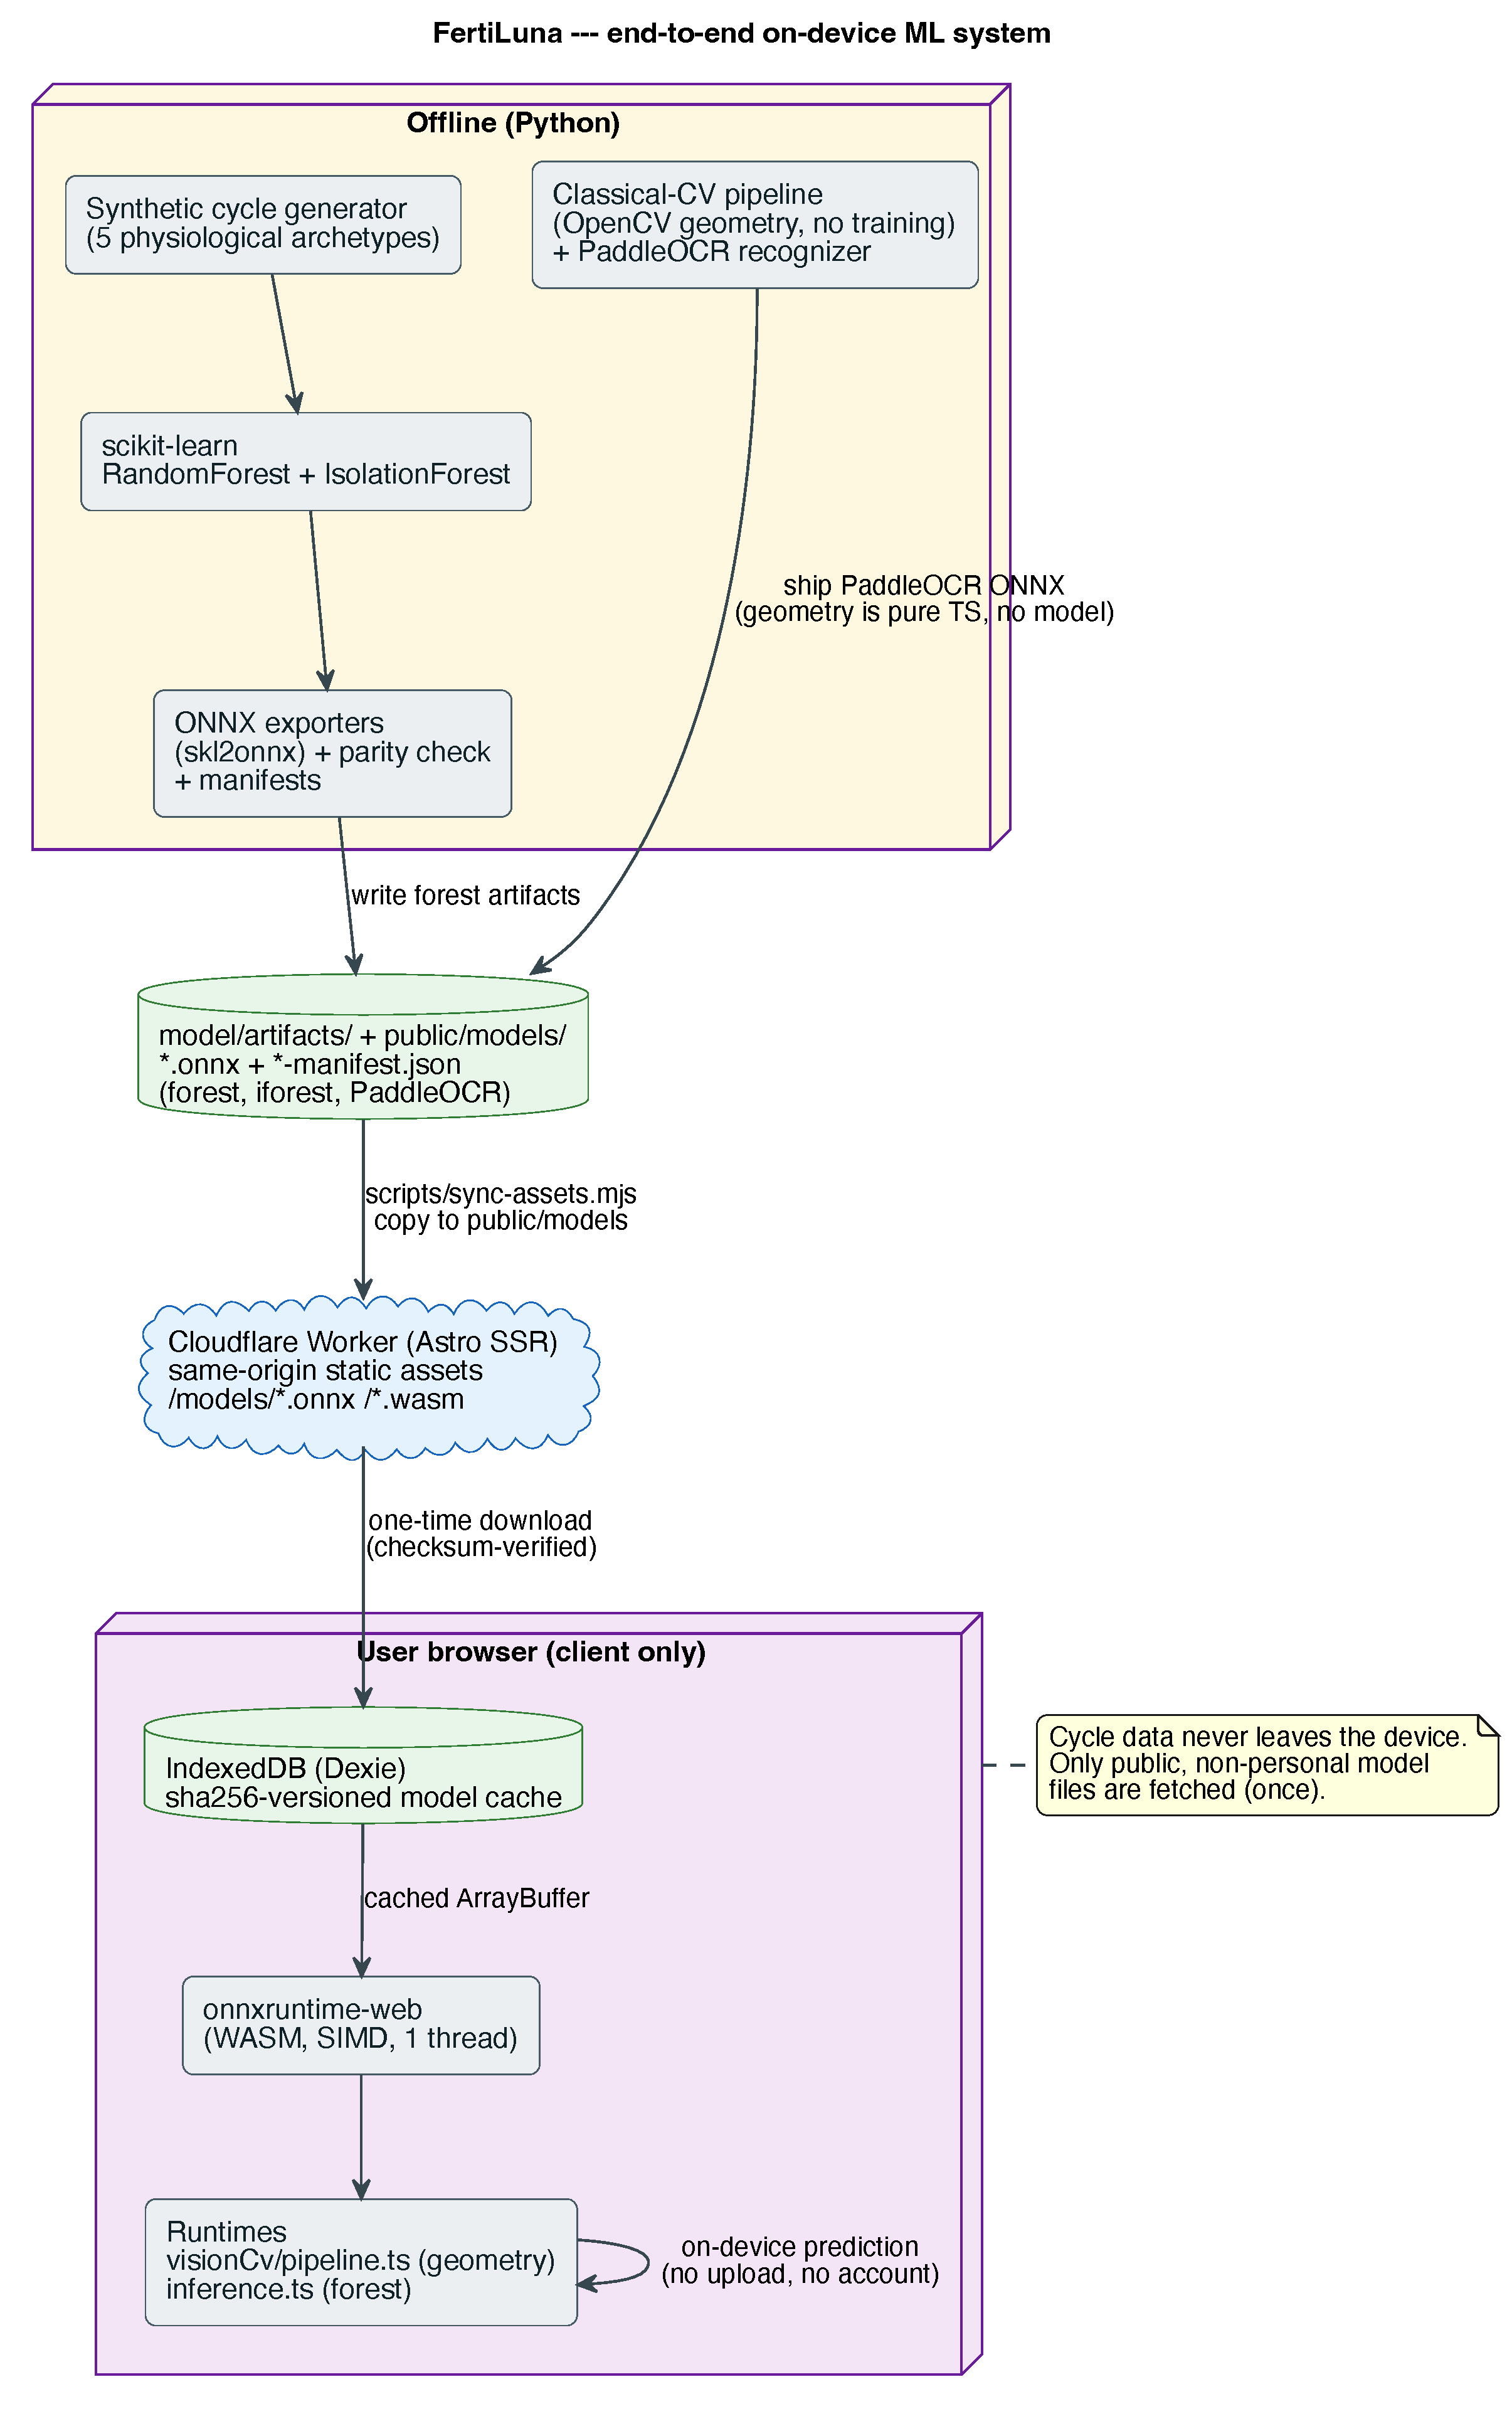
\includegraphics[width=0.93\textwidth]{figures/system-architecture.pdf}
\caption{End-to-end system architecture. Training is offline; serving is a
same-origin static-asset delivery; all inference is client-side. The dashed
boundary around the browser denotes the privacy perimeter: cycle data never
crosses it.}
\label{fig:sysarch}
\end{figure}

\subsection{Technology stack}
The application is written in TypeScript and Astro and deployed on Cloudflare
Workers (server-side rendering for the page shell only). Browser inference uses
\code{onnxruntime-web} on the WASM backend with a single thread and SIMD enabled,
which avoids the cross-origin-isolation (\code{COOP}/\code{COEP}) headers that
multi-threaded WASM would require. The model cache is built on Dexie (a typed
wrapper over IndexedDB). The Python side uses NumPy, pandas, and scikit-learn for
the forest family~\cite{pedregosa2011scikit}; PyTorch for the vision network;
and \code{skl2onnx}/\code{torch.onnx} for export~\cite{onnx2017,skl2onnx}.

%==============================================================================
\section{The forest model: calibrated cycle classification}
\label{sec:forest}
%==============================================================================

\subsection{Problem formulation}
Let a cycle be represented by two length-$D$ vectors ($D = 35$ days),
$\bm{t} \in (\mathbb{R}\cup\{\textsc{nan}\})^{D}$ of temperatures and
$\bm{\ell}$ of LH values, where \textsc{nan} marks a missing observation. A
deterministic feature map $\phi$ produces a fixed vector
$\bm{x} = \phi(\bm{t},\bm{\ell}) \in \mathbb{R}^{30}$, and a classifier assigns
one of five labels:
\[
\mathcal{Y} = \{
\text{\small ovulation\_confirmee},\
\text{\small ovulation\_douteuse},\
\text{\small anovulation},\
\text{\small phase\_luteale\_courte},\
\text{\small donnees\_insuffisantes}
\}.
\]
These correspond, respectively, to a confirmed ovulation, a doubtful thermal
shift, an anovulatory cycle, a short luteal phase, and insufficient data.

\subsection{Feature engineering}
\label{sec:features}
The thirty features (Table~\ref{tab:features}) are scalar, NaN-safe summaries
of the two curves. The design philosophy is to hand the model the same
quantities a clinician would inspect, so that the learned function refines
domain knowledge rather than rediscovering it from scratch. The cornerstone
is a hard-coded implementation of the SENSIPLAN 3-over-6 ovulation rule: the
first day $d$ at which three consecutive temperatures strictly exceed the
maximum of the preceding six, with the third exceeding that maximum by at
least \SI{0.2}{\celsius}, marks the last follicular day.

\begin{lstlisting}[language=Python,caption={The SENSIPLAN 3-over-6 detector, the
anchor feature for follicular/luteal partitioning (from \file{features.py}).}]
def _detect_ovulation_day_sensiplan(temps):
    n = len(temps)
    for d in range(6, n - 2):
        prior  = temps[d - 6 : d]
        rising = temps[d : d + 3]
        prior_max = float(np.nanmax(prior))
        if not np.all(rising > prior_max):
            continue
        if rising[2] - prior_max < 0.20:        # >= 0.2 C confirmation
            continue
        return d - 1                            # last follicular day (0-indexed)
    return -1
\end{lstlisting}

\begin{table}[H]
\centering
\caption{The thirty-dimensional feature vector $\phi(\bm{t},\bm{\ell})$.
Indices match \file{constants.py}. All entries are scalars; missing days
contribute \textsc{nan} that is handled by NaN-safe reductions.}
\label{tab:features}
\small
\begin{adjustbox}{max width=\textwidth}
\begin{tabular}{@{}rl rl rl@{}}
\toprule
\# & Feature & \# & Feature & \# & Feature\\
\midrule
0  & \code{n\_temp\_observed}        & 10 & \code{follicular\_mean}            & 20 & \code{lh\_peak\_value}\\
1  & \code{n\_lh\_observed}          & 11 & \code{follicular\_std}             & 21 & \code{lh\_peak\_count}\\
2  & \code{missing\_rate\_temp}      & 12 & \code{luteal\_mean}                & 22 & \code{days\_lh\_peak\_to\_rise}\\
3  & \code{missing\_rate\_lh}        & 13 & \code{luteal\_std}                 & 23 & \code{follicular\_length}\\
4  & \code{temp\_mean\_overall}      & 14 & \code{thermal\_rise\_amplitude}    & 24 & \code{luteal\_length}\\
5  & \code{temp\_std\_overall}       & 15 & \code{rise\_steepness\_max}        & 25 & \code{slope\_pre\_ovulation}\\
6  & \code{temp\_min}                & 16 & \code{plateau\_days\_above\_base}  & 26 & \code{slope\_post\_ovulation}\\
7  & \code{temp\_max}                & 17 & \code{n\_consecutive\_high\_days}  & 27 & \code{fraction\_days\_below\_mean}\\
8  & \code{temp\_range}              & 18 & \code{post\_rise\_dip\_count}      & 28 & \code{longest\_run\_above\_mean}\\
9  & \code{estimated\_ovulation\_day}& 19 & \code{lh\_peak\_day}               & 29 & \code{longest\_run\_below\_mean}\\
\bottomrule
\end{tabular}
\end{adjustbox}
\end{table}

\subsection{Synthetic data generation}
No real labeled corpus exists at the scale required, and collecting one would
contradict the privacy thesis. We therefore generate
$N = \num{50000}$ physiologically grounded cycles from five archetypes with
prior weights $(0.45, 0.15, 0.15, 0.15, 0.10)$ for
\{normal, doubtful, short-luteal, anovulation, insufficient\}. Each archetype
samples plausible parameters (follicular and luteal lengths, thermal-rise
amplitude and duration, baseline temperature, measurement noise), and the
curve is then corrupted with realistic artifacts (fever bumps,
late-measurement spikes) and missing data. The LH surge is placed
\numrange{12}{36} hours before ovulation, with optional spurious peaks that
emulate PCOS-like patterns. Labels are assigned by the same clinical rules
the model is meant to internalize, so the classifier learns a noise-robust
version of an explicit decision procedure.

\subsection{Model and calibration}
The classifier is a \code{RandomForestClassifier}~\cite{breiman2001random}
with \num{120} trees, maximum depth \num{12}, minimum leaf size \num{12},
$\sqrt{\cdot}$ feature subsampling, and balanced class weights. Raw
random-forest probabilities are poorly calibrated. They cluster near the
extremes, which would make a fixed confidence threshold meaningless. We
therefore apply Platt (sigmoid) calibration
\cite{platt1999probabilistic,niculescu2005predicting}.

A subtle but important engineering decision concerns \emph{how} calibration
is fitted. The default \code{CalibratedClassifierCV(cv=5)} trains five
separate forests, which would serialize to roughly \SI{250}{\mega\byte} of
ONNX. That is a non-starter for a browser download. Instead we train a
\emph{single} forest on a ``fit'' split and calibrate it on a held-out
``calibration'' split using a frozen (prefit) estimator. The exported graph
thus contains exactly one tree ensemble (\SI{5.6}{\mega\byte}) while still
yielding the calibrated probabilities the confidence gate relies upon.

\begin{lstlisting}[language=Python,caption={Single prefit forest, calibrated on a
held-out split (from \file{train.py}).}]
base_rf = RandomForestClassifier(n_estimators=120, max_depth=12,
                                 min_samples_leaf=12, max_features="sqrt",
                                 class_weight="balanced", random_state=seed)
base_rf.fit(X_fit, y_fit)                       # ONE forest
clf = CalibratedClassifierCV(estimator=FrozenEstimator(base_rf),
                             method="sigmoid")   # Platt scaling only
clf.fit(X_calib, y_calib)
\end{lstlisting}

At inference time the predicted label is the $\argmax$ of the calibrated
probabilities, \emph{unless} the maximum probability falls below the gate
$\tau = 0.60$, in which case the label is overridden to
\textsc{donnees\_insuffisantes}:
\begin{equation}
\hat{y} =
\begin{cases}
\argmax_k p_k & \text{if } \max_k p_k \ge \tau,\\[2pt]
\text{\small donnees\_insuffisantes} & \text{otherwise.}
\end{cases}
\label{eq:gate}
\end{equation}

\subsection{Out-of-distribution detection}
A classifier trained on synthetic archetypes will happily produce confident,
yet meaningless, outputs on genuinely anomalous curves. As an advisory
backstop we fit an isolation forest~\cite{liu2008isolation} with \num{150}
estimators and contamination \num{0.10} on the same features, and store the
$5^{\text{th}}/50^{\text{th}}/95^{\text{th}}$ percentiles of its
decision-function on the training distribution. At run time a raw anomaly
score $s$ is mapped to a $0$--$100$ ``unusualness'' percentile by
piecewise-linear interpolation through those anchors (lower $s$
$\Rightarrow$ more anomalous), and surfaced in the UI rather than used to
alter the label.

\subsection{Training and export pipeline}
Figure~\ref{fig:forest} renders the complete pipeline. After export,
\code{skl2onnx}~\cite{skl2onnx} produces graphs pinned to opset~17 (and
\code{ai.onnx.ml}~3, the version supported by ONNX Runtime Web). A parity check
asserts that the maximum absolute difference between scikit-learn and ONNX Runtime
probabilities is below $10^{-3}$; in practice it is $\approx\! 1.2\times10^{-7}$.

\begin{figure}[H]
\centering
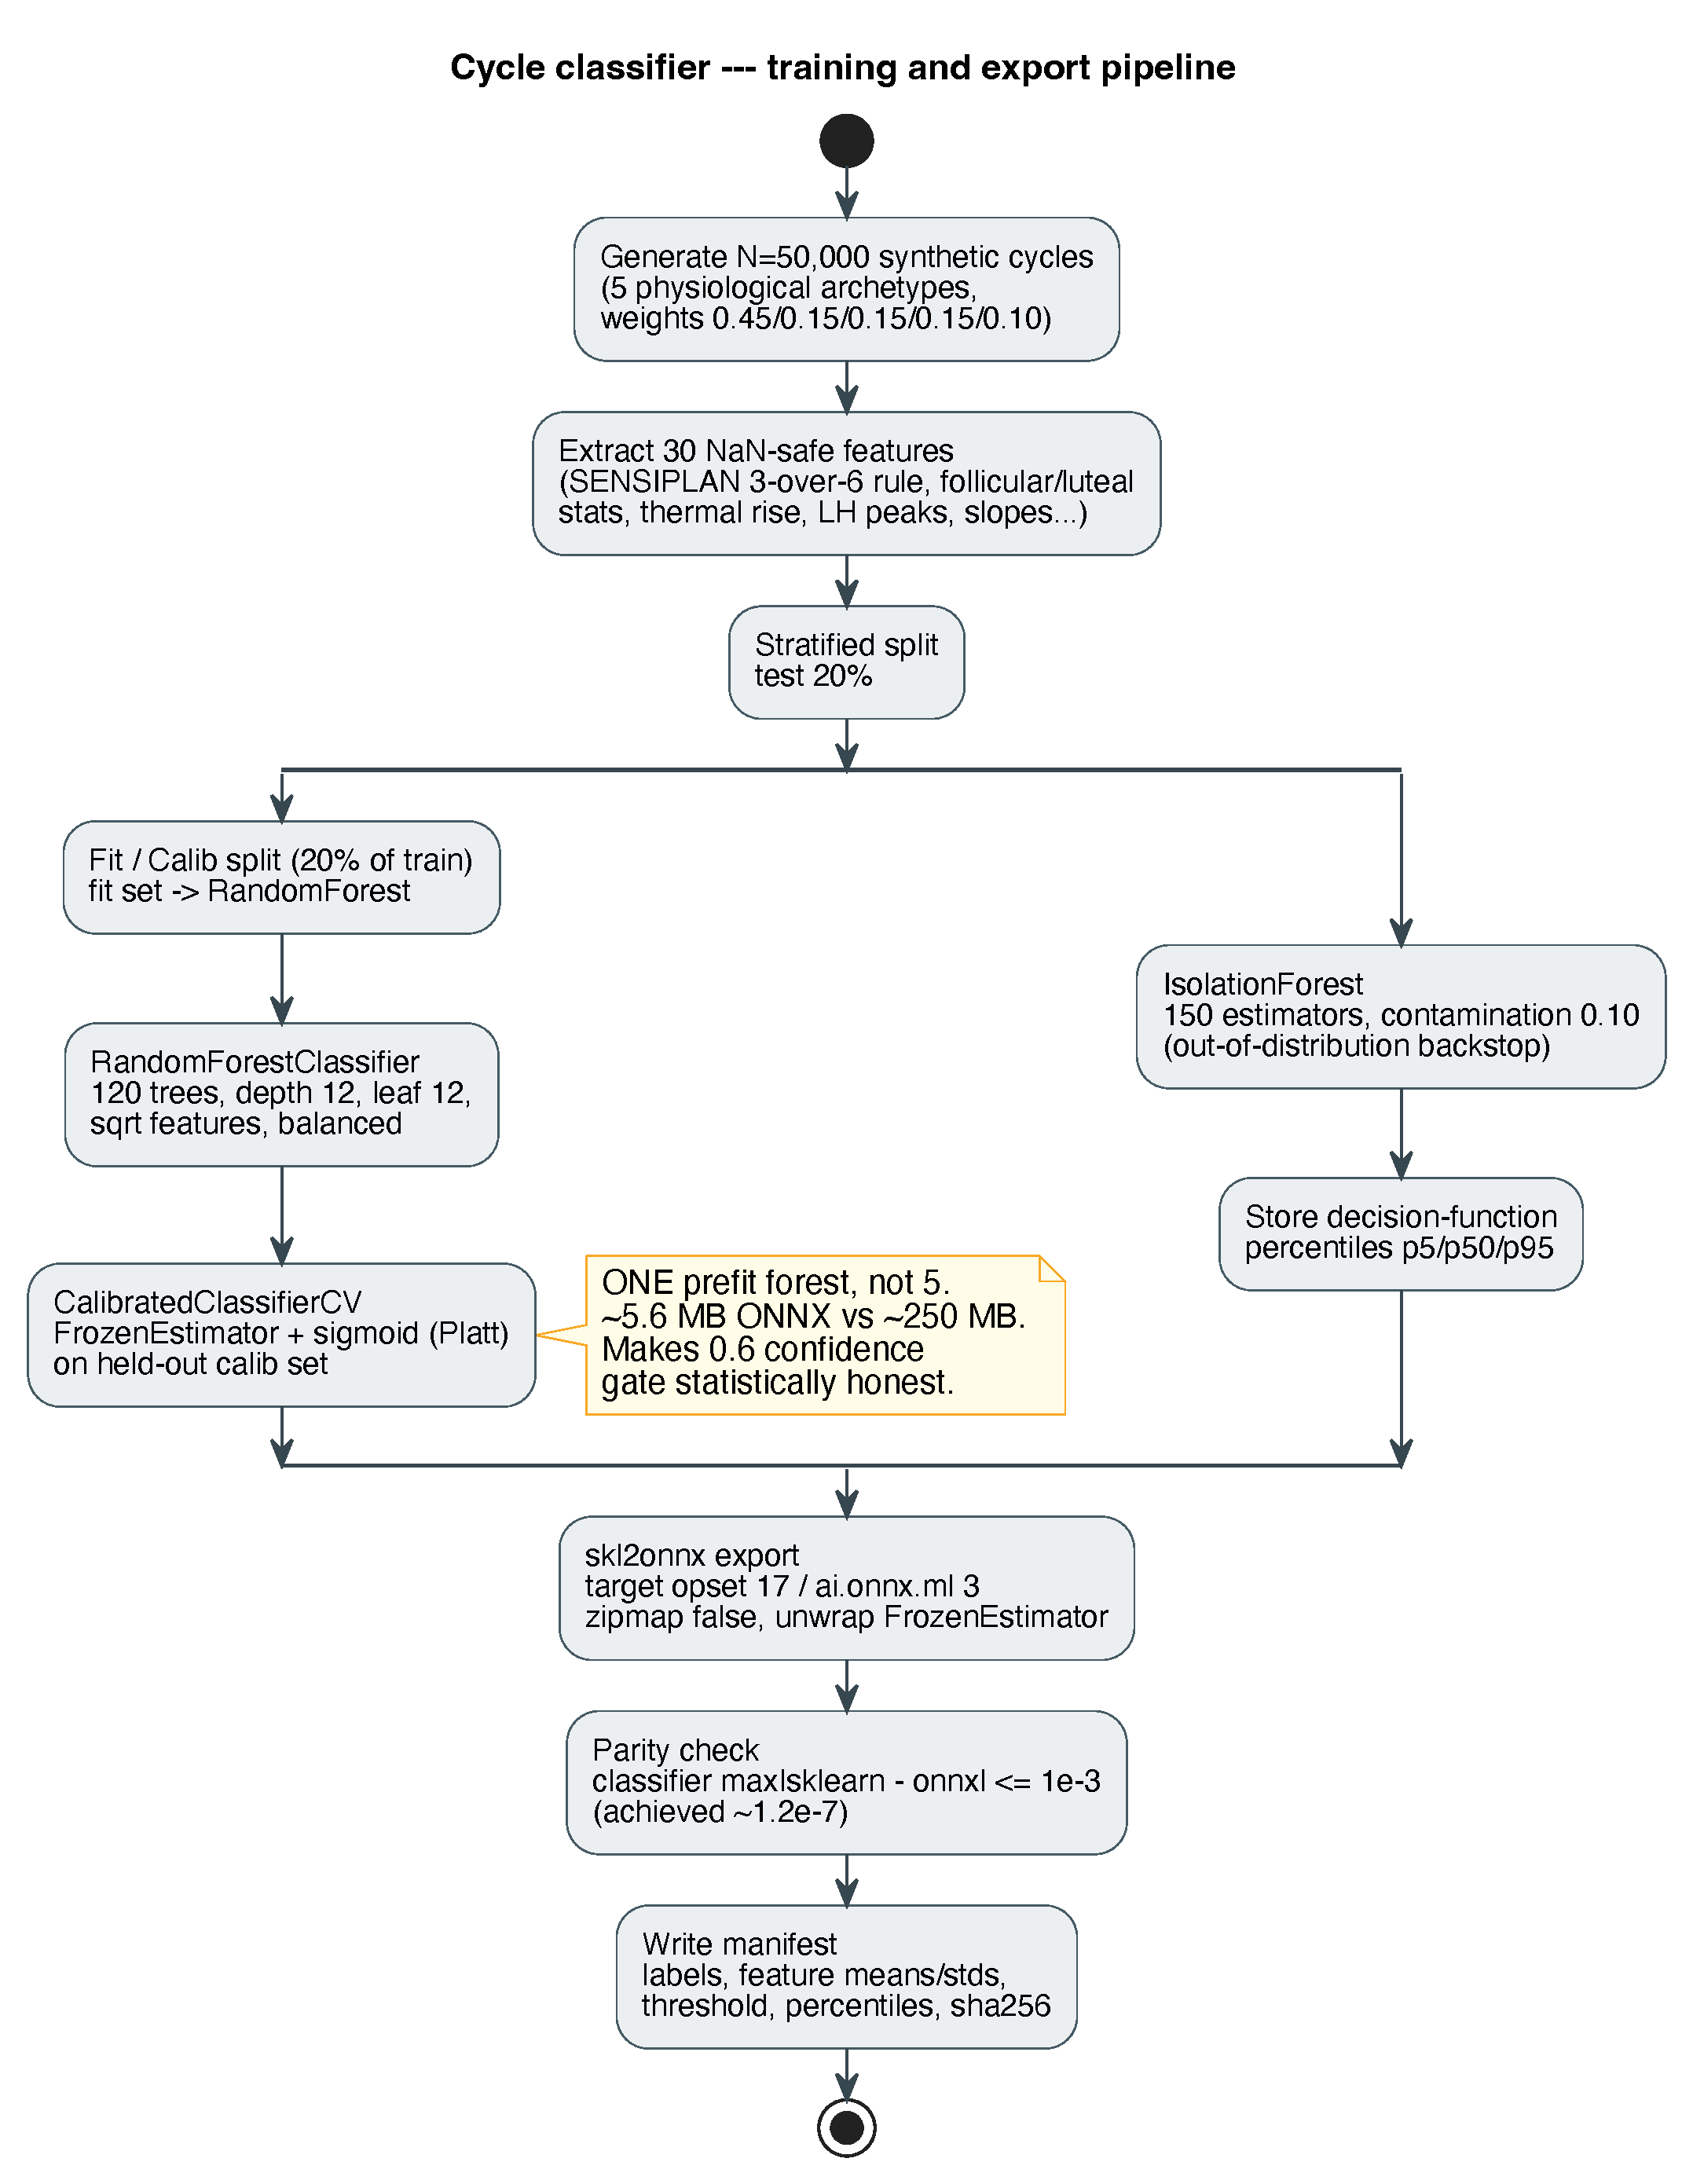
\includegraphics[height=0.86\textheight]{figures/forest-pipeline.pdf}
\caption{Forest training and export pipeline: synthetic generation, feature
extraction, a single prefit forest with Platt calibration, an isolation-forest
OOD backstop, and ONNX export with an enforced numerical-parity contract.}
\label{fig:forest}
\end{figure}

\subsection{Results}
On a held-out synthetic test set of \num{10000} cycles the calibrated
classifier reaches an accuracy of \SI{88.56}{\percent} and a log loss of
\num{0.329}. Per-class metrics appear in Table~\ref{tab:forestmetrics}; the
confusion matrix is visualized in Figure~\ref{fig:cm}. As expected, the
main confusions live between \emph{confirmed} and \emph{doubtful} ovulation
and between \emph{doubtful} and \emph{short-luteal}. These are boundaries
that are genuinely fuzzy in clinical practice. The data-sufficiency and
anovulation classes, on the other hand, are recovered cleanly.

\begin{table}[H]
\centering
\caption{Per-class performance of the calibrated forest on the synthetic test set
($n=\num{10000}$).}
\label{tab:forestmetrics}
\small
\begin{tabular}{@{}lS[table-format=1.3]S[table-format=1.3]S[table-format=1.3]S[table-format=4.0]@{}}
\toprule
Class & {Precision} & {Recall} & {$F_1$} & {Support}\\
\midrule
ovulation\_confirmee   & 0.957 & 0.932 & 0.944 & 4474\\
ovulation\_douteuse    & 0.764 & 0.784 & 0.774 & 1495\\
anovulation            & 0.876 & 0.877 & 0.876 & 1507\\
phase\_luteale\_courte & 0.784 & 0.828 & 0.805 & 1526\\
donnees\_insuffisantes & 0.939 & 0.933 & 0.936 & 998\\
\midrule
\textbf{Accuracy} & \multicolumn{4}{r}{\textbf{0.8856} \quad (log loss \textbf{0.329})}\\
\bottomrule
\end{tabular}
\end{table}

\begin{figure}[H]
\centering
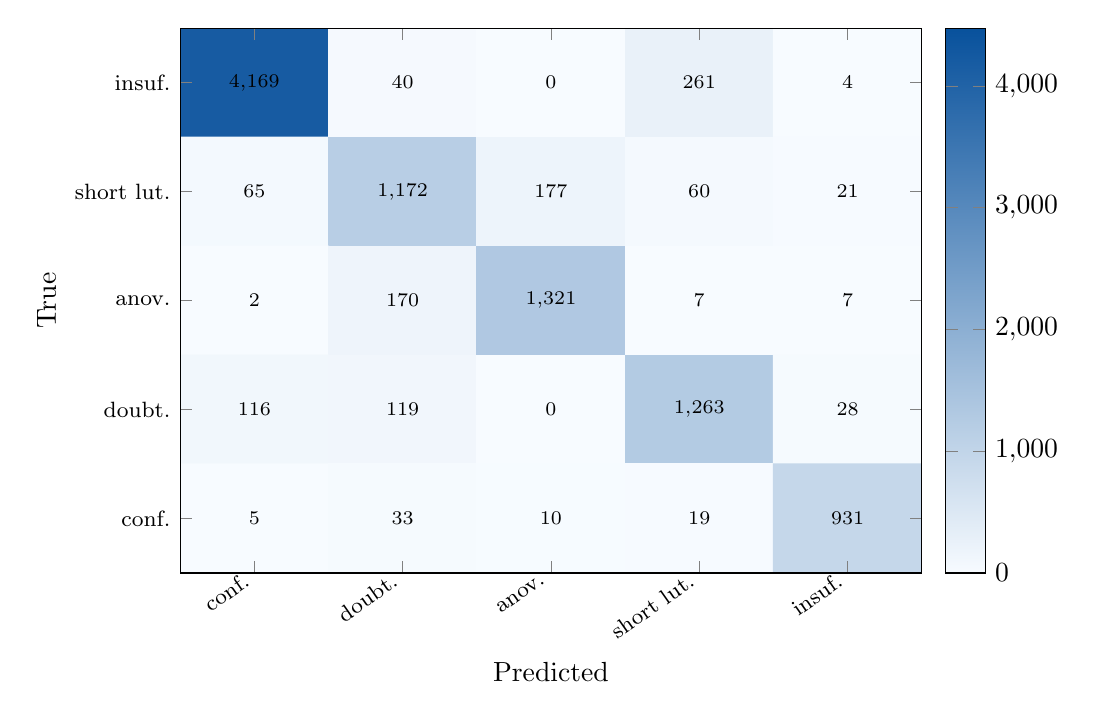
\begin{tikzpicture}
\begin{axis}[
  width=11cm, height=8.5cm,
  enlargelimits=false, axis on top,
  colormap={blues}{rgb255=(247,251,255) rgb255=(8,81,156)},
  colorbar, point meta min=0, point meta max=4474,
  xtick={0,1,2,3,4}, ytick={0,1,2,3,4},
  xticklabels={conf.,doubt.,anov.,short lut.,insuf.},
  yticklabels={conf.,doubt.,anov.,short lut.,insuf.},
  xticklabel style={rotate=35,anchor=east,font=\footnotesize},
  yticklabel style={font=\footnotesize},
  xlabel={Predicted}, ylabel={True},
  nodes near coords align={anchor=center},
]
\addplot[matrix plot*,point meta=explicit,mesh/cols=5,
  nodes near coords={\pgfmathprintnumber\pgfplotspointmeta},
  every node near coord/.append style={font=\scriptsize,
    /pgf/number format/precision=0,/pgf/number format/fixed}]
table[meta=C] {
x y C
0 4 4169
1 4 40
2 4 0
3 4 261
4 4 4
0 3 65
1 3 1172
2 3 177
3 3 60
4 3 21
0 2 2
1 2 170
2 2 1321
3 2 7
4 2 7
0 1 116
1 1 119
2 1 0
3 1 1263
4 1 28
0 0 5
1 0 33
2 0 10
3 0 19
4 0 931
};
\end{axis}
\end{tikzpicture}
\caption{Confusion matrix of the calibrated forest (rows: true class top-to-bottom
follows the legend order; counts annotated). The dominant off-diagonal mass lies
between adjacent clinical categories.}
\label{fig:cm}
\end{figure}

%==============================================================================
\section{The vision stage: reading charts with classical computer vision}
\label{sec:vision}
%==============================================================================

\subsection{Problem statement}
Many users arrive with a screenshot from an existing fertility app rather
than a table of numbers. The vision stage recovers, from a single RGB image,
two per-day series (basal body temperature, BBT, and the LH or
ovulation-test signal), together with the temperature unit of the BBT axis
(Celsius or Fahrenheit) and an auxiliary parse of the calendar table beneath
the chart. Its output is exactly the structured representation that the
forest classifier of Section~\ref{sec:forest} consumes, so the two stages
compose cleanly.

\subsection{Why a deterministic pipeline rather than a neural network}
\label{sec:why-cv}
We implemented \emph{two} solutions to this problem: a convolutional neural
network (described, for completeness, in Section~\ref{sec:cnn-alt}) and a
\emph{classical computer-vision pipeline} built on OpenCV. \textbf{The
deployed vision stage is the classical pipeline.} The neural network is
kept as a research baseline but is not shipped. The decision rests on four
properties that matter more than raw accuracy for a privacy-first,
on-device health tool:

\begin{enumerate}
  \item \textbf{Determinism and auditability.} Every decision in the
  pipeline is an explicit, inspectable rule with a named constant (an HSV
  band, a coverage threshold, a RANSAC tolerance). There are no learned
  weights to reason about, no opaque failure modes, and the same input
  always yields the same output. For a tool that informs reproductive
  decisions, an auditable extraction is preferable to a marginally more
  accurate black box.
  \item \textbf{Structured side-output for free.} Because the pipeline
  reasons about the image geometrically, it also recovers the axis tick
  \emph{values}, the day-cell grid, the detected markers, and the bottom
  calendar table (cycle-day, days-past-ovulation, intercourse,
  cervical-mucus, hCG). The CNN produces only the two series and the unit;
  the table would require a separate model.
  \item \textbf{No training data, no sim-to-real gap.} The CNN must be
  trained on procedurally rendered charts and then bridged to real app
  screenshots. The classical pipeline reads the real screenshot directly,
  so there is no distribution shift to manage.
  \item \textbf{Smaller and simpler to ship.} The only model asset the
  pipeline needs is a \SI{\sim 9}{\mega\byte} PaddleOCR text-recognition
  network used to read axis labels~\cite{du2020ppocr}; the geometry is pure
  arithmetic. The CNN would add a \SI{16.6}{\mega\byte} download with no
  table output.
\end{enumerate}

The one genuine cost is engineering effort: the pipeline is a sequence of
hand-tuned stages, whereas the CNN is a single trained artifact. We judged
that cost worthwhile, given the auditability and side-output benefits.

\subsection{Pipeline architecture}
\label{sec:cvarch}
The pipeline (Figure~\ref{fig:cvpipeline}) is an ordered sequence of nine stages
implemented in Python with OpenCV and NumPy, plus a PaddleOCR PP-OCRv3 recognizer
exported to ONNX for reading axis tick labels. The same stages are mirrored, op
for op, in a pure-TypeScript browser port (Section~\ref{sec:cv-browser}) so that
the production tool runs entirely client-side. Each stage consumes the working
image and the accumulated state and contributes to a single \code{ChartResult}.

\begin{figure}[H]
\centering
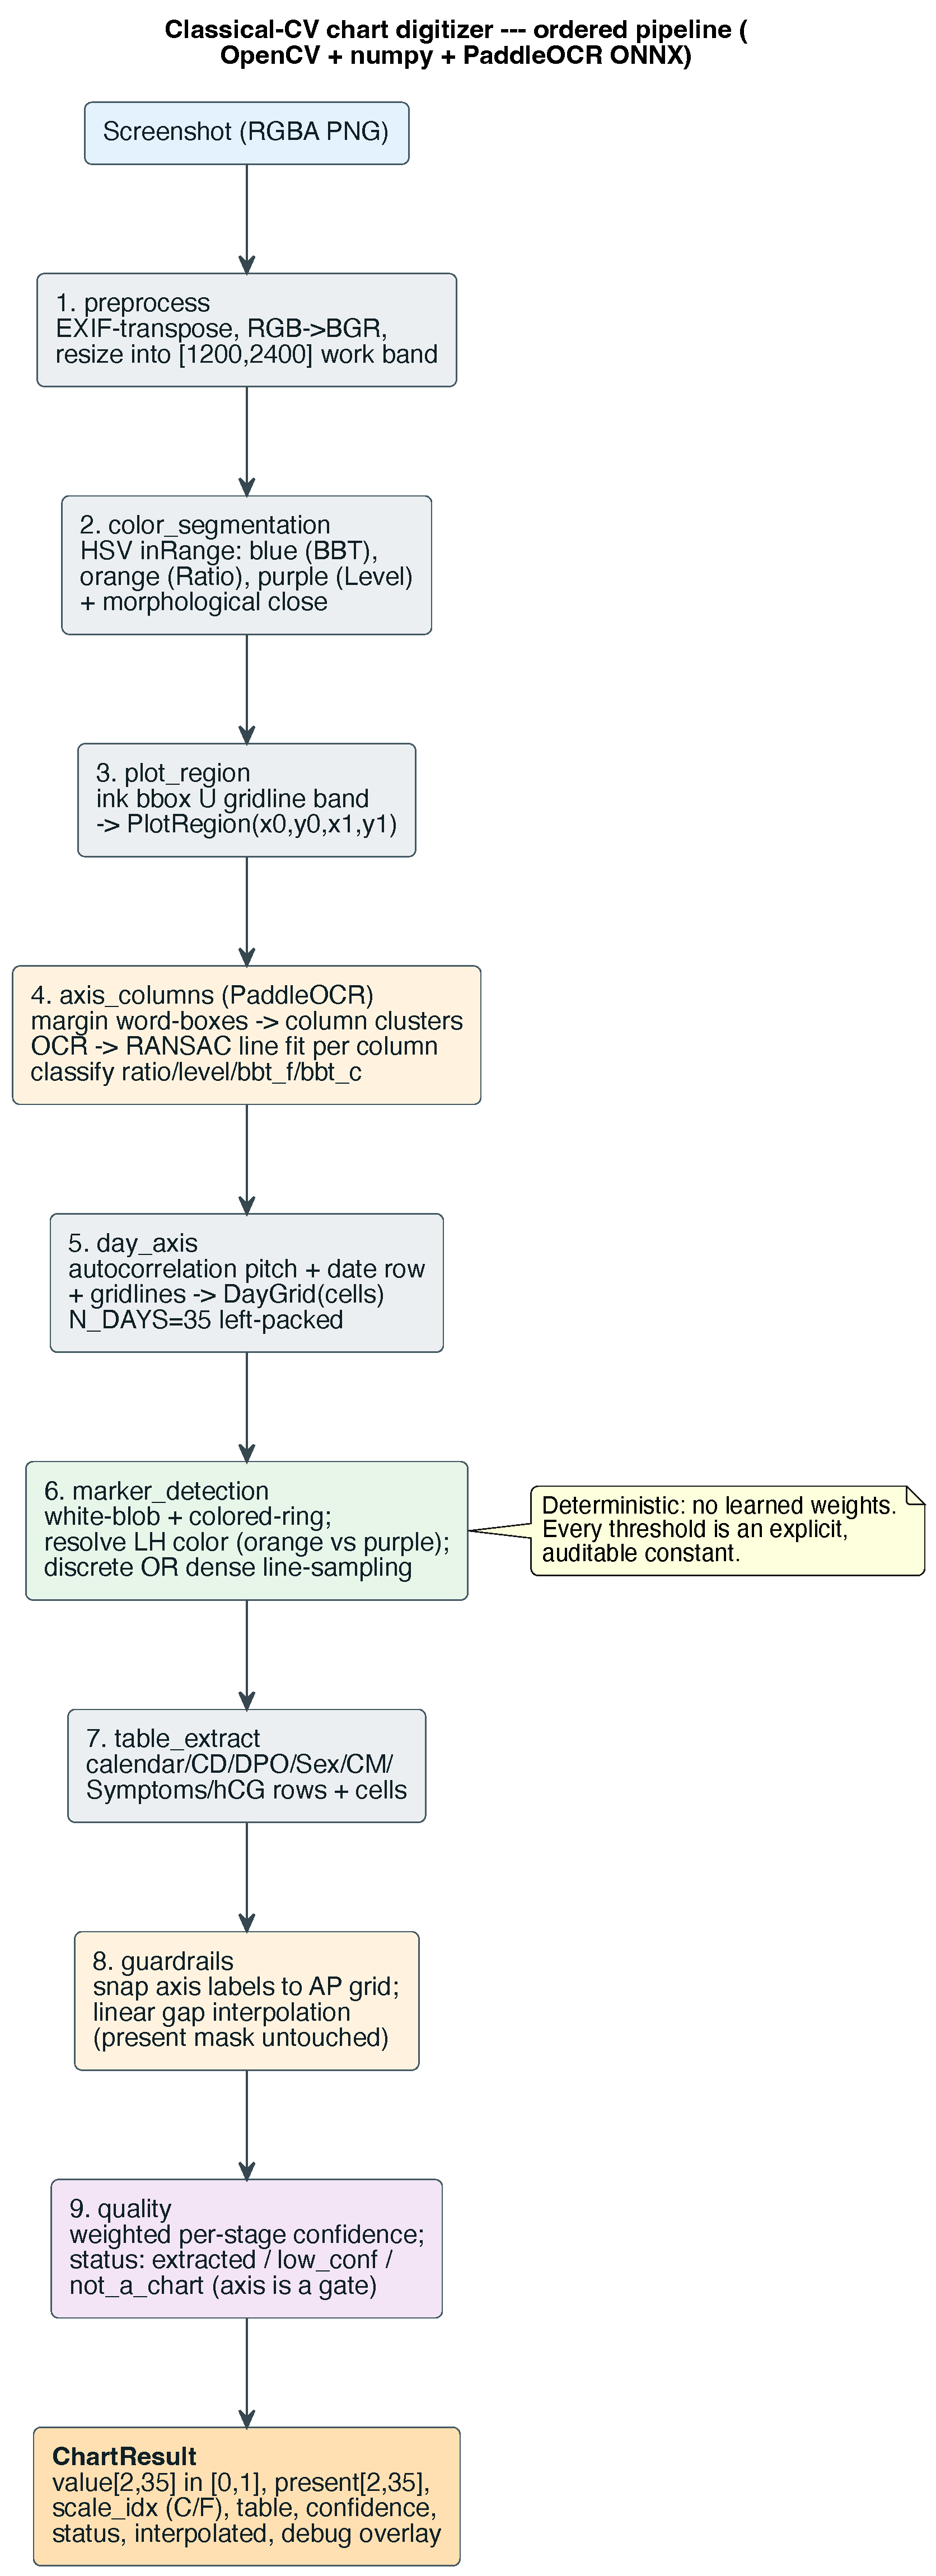
\includegraphics[height=0.83\textheight]{figures/cv-pipeline.pdf}
\caption{The classical-CV chart digitizer: nine ordered, deterministic stages
from raw screenshot to \code{ChartResult}. The only learned component is a small
PaddleOCR network that reads numeric axis labels; all geometry is explicit
arithmetic.}
\label{fig:cvpipeline}
\end{figure}

\subsection{Key stages in detail}

\paragraph{Color segmentation (stage 2).}
The chart's series are distinguished by color, so the pipeline converts to
HSV and applies deliberately \emph{non-overlapping} \code{inRange} bands:
blue for BBT, orange for the LH ``Ratio'' line, and purple for the LH
``Level'' line. The non-overlap is a design choice: it guarantees that the
purple distractor cannot leak into the blue BBT mask. A small morphological
close bridges the gaps between line strokes.

\paragraph{Multi-axis tick reading via OCR $+$ RANSAC (stage 4).}
This is the heart of unit detection and de-normalization. Premom-style
charts carry up to three stacked $y$-axes (a Ratio axis, a Level axis, and
the BBT axis). The pipeline detects text word-boxes in the left and right
margins, clusters them into vertical \emph{columns} by their $x$-center,
OCRs each box with PaddleOCR, and fits a line $\text{value} = a + b\,y$ to
each column by RANSAC. RANSAC keeps the fit robust to a stray calendar
date that leaks into the margin. Each fitted column is then classified by
matching its top/bottom value span against known axis profiles:
\[
\text{ratio}\,(1.9{\to}0.1),\quad
\text{level}\,(95{\to}5),\quad
\text{bbt}_{\text{F}}\,(99.5{\to}95),\quad
\text{bbt}_{\text{C}}\,(37.4{\to}35.6).
\]
Crucially, the temperature unit is read \emph{directly} from which BBT
column exists, rather than guessed. If a column fits the $[95,99.5]$
Fahrenheit profile, the scale is Fahrenheit with full confidence. The
inverse of the fitted line, $\text{value\_at}(y) = a + b\,y$, later maps
each detected marker's pixel position to a physical value.

\paragraph{Day-cell grid (stage 5).}
The horizontal day axis is recovered, in priority order, by clustering the
date-row digits, by detecting vertical gridlines, or, failing those, by
taking the dominant pitch of the column-density autocorrelation and
cross-checking it against the marker spacing. The grid is constrained to a
plausible pitch and coverage, and tiled to $N\!=\!35$ cells anchored at the
leftmost marker. Charts that show more than 35 days are left-packed and
flagged \code{truncated}.

\paragraph{Marker detection and LH-source resolution (stage 6).}
Data points are small white blobs ringed by a colored stroke. The detector finds
white connected components inside the plot and, for each, sweeps candidate ring
radii and measures the fraction of an angular sample that falls on each color
mask; the best-covered color assigns the blob to a series. A dedicated step
resolves whether the LH signal is carried by the orange ``Ratio'' line or the
purple ``Level'' line by comparing discrete-marker counts and ink continuity.
For dense, near-continuous curves the detector switches from discrete markers to
per-cell line sampling, reading the ink centroid in each day column while
excluding the flat BBT threshold line.

\paragraph{Guardrails (stage 8).}
Two repairs run before the result is emitted. First, OCR labels are snapped
onto the inferred arithmetic tick grid (the canonical fix
$[36, \texttt{"5"}, 37] \rightarrow [36, 36.5, 37]$). Second, short gaps in
each series are linearly interpolated, but the \code{present} mask is
\emph{never} modified, so a synthesised day can never be mistaken for a
measured one. This separation is a deliberate medical-safety property.

\paragraph{Quality gating (stage 9).}
A weighted confidence in $[0,1]$ is computed from per-stage signals, and the
fitted BBT axis acts as a gate: with no trustworthy axis the marker contribution
is heavily discounted and the status is capped at \emph{low confidence}; with no
axis and fewer than two points the image is rejected as \emph{not a chart}.

\subsection{The \texttt{ChartResult} contract}
The pipeline emits a single dataclass whose numeric core is identical to the
schema the neural alternative would produce, so downstream code is agnostic to
which vision stage ran (Table~\ref{tab:chartresult}).

\begin{table}[H]
\centering
\caption{The principal fields of \code{ChartResult}. The numeric core
(\code{value}, \code{present}, \code{scale\_idx}) matches the contract of the
neural alternative; the remaining fields are side-outputs unique to the
geometric pipeline.}
\label{tab:chartresult}
\small
\begin{adjustbox}{max width=\textwidth}
\begin{tabular}{@{}lll@{}}
\toprule
Field & Type & Meaning\\
\midrule
\code{value}        & $(2,35)$ float32 & per-series value, normalized to $[0,1]$ within its axis range\\
\code{present}      & $(2,35)$ float32 & measured-day mask $\in\{0,1\}$ (never inferred)\\
\code{scale\_idx}   & int              & $0=$ Celsius, $1=$ Fahrenheit\\
\code{scale\_label}, \code{scale\_confidence} & str, float & detected unit and its confidence\\
\code{table}        & dict             & calendar / CD / DPO / Sex / CM / Symptoms / hCG rows and cells\\
\code{visible\_days}, \code{truncated} & int, bool & estimated days shown; flag when $>35$\\
\code{confidence}, \code{status} & float, str & overall quality and \{extracted, low\_confidence, not\_a\_chart\}\\
\code{interpolated} & $(2,35)$ float32 & $1.0$ on synthesised days (kept separate from \code{present})\\
\code{debug}        & dict             & masks, plot box, grid, axis columns, markers (drives the overlay)\\
\bottomrule
\end{tabular}
\end{adjustbox}
\end{table}

\subsection{Results on real Premom screenshots}
\label{sec:cvresults}
We evaluate the pipeline on four real, in-the-wild Premom screenshots that differ
in language, temperature unit, chart density, and LH source. The pipeline is run
through its command-line \emph{assess} mode, which renders a diagnostic overlay
and emits the decoded JSON:
\begin{lstlisting}[language=bash,caption={Producing the diagnostic overlays from
real screenshots (run from \file{model/}).}]
python -m fertiluna_vision_cv.cli assess \
    --images ../real-screen-1.png ../real-screen-2.png \
             ../real-screen-3.png ../real-screen-4.png \
    --out /tmp/cv-assess
# -> {stem}_overlay.png + {stem}_decoded.json + index.html
\end{lstlisting}

\noindent
Table~\ref{tab:cvreal} summarizes the per-screenshot outcome. The unit is
auto-detected correctly in every case (Celsius for the German screenshot,
Fahrenheit for the others), the LH source is correctly resolved between the
orange and purple lines, and the two long charts ($\approx 42$ visible days) are
correctly flagged as truncated.

\begin{table}[H]
\centering
\caption{Classical-CV pipeline on four real Premom screenshots. Counts are
detected (present) days out of the 35-day window; \emph{vis.} is the estimated
number of days the chart actually shows.}
\label{tab:cvreal}
\small
\begin{adjustbox}{max width=\textwidth}
\begin{tabular}{@{}llcccccc@{}}
\toprule
Screenshot & Description & Scale (conf.) & LH source & BBT & LH & Vis. / trunc. & Status (conf.)\\
\midrule
real-screen-1 & English, sparse       & F\,(1.00) & orange ``Ratio'' & 16/35 & 15/35 & 18 / no  & extracted (0.87)\\
real-screen-2 & German, sparse        & C\,(0.80) & orange ``Ratio'' & 19/35 & 19/35 & 25 / no  & extracted (0.71)\\
real-screen-3 & dense ($\approx$42 d) & F\,(1.00) & purple ``Level'' & 34/35 & 35/35 & 42 / yes & extracted (0.83)\\
real-screen-4 & dense $+$ LH peak     & F\,(1.00) & purple ``Level'' & 35/35 & 35/35 & 42 / yes & extracted (0.82)\\
\bottomrule
\end{tabular}
\end{adjustbox}
\end{table}

The diagnostic overlay drawn by the pipeline (\code{debug\_overlay.py}) is the
clearest way to see what each stage recovered. It draws the detected plot region
(green), the axis tick boxes labeled with their OCR'd values and classified kind
(ratio / level / bbt), the day-cell grid (numbered $1$--$35$), the BBT markers
(blue rings) and LH markers (orange rings), and the extracted calendar table,
with a per-day decoded value strip beneath. Figures~\ref{fig:overlay1}
and~\ref{fig:overlay3} show two contrasting cases.

\begin{figure}[H]
\centering
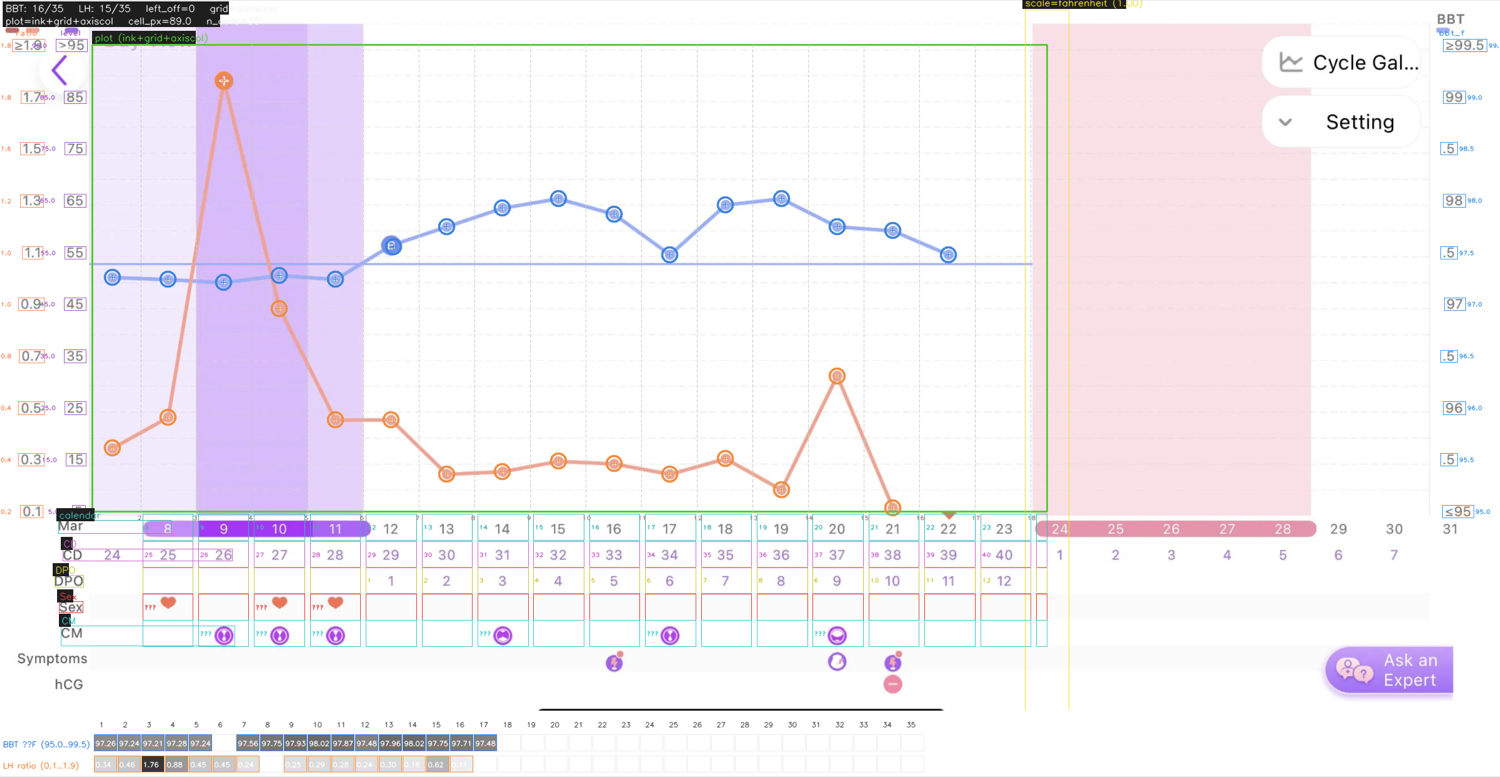
\includegraphics[width=\textwidth]{figures/overlays/overlay-1.png}
\caption{Overlay for \texttt{real-screen-1} (English, sparse, Fahrenheit
auto-detected). Blue rings are detected BBT points; orange rings are the LH
``Ratio'' line; the green box is the plot region; the numbered ticks at the
bottom are the day-cell grid; the right-margin boxes are the OCR'd Fahrenheit BBT
axis ($\geq\!95$ \dots $\geq\!99.5$); the bottom rows are the recovered calendar
table (Mar dates, CD, DPO, Sex hearts, CM). The two-row strip at the very bottom
is the de-normalized output (\si{\degree F} for BBT, ratio for LH).}
\label{fig:overlay1}
\end{figure}

\begin{figure}[H]
\centering
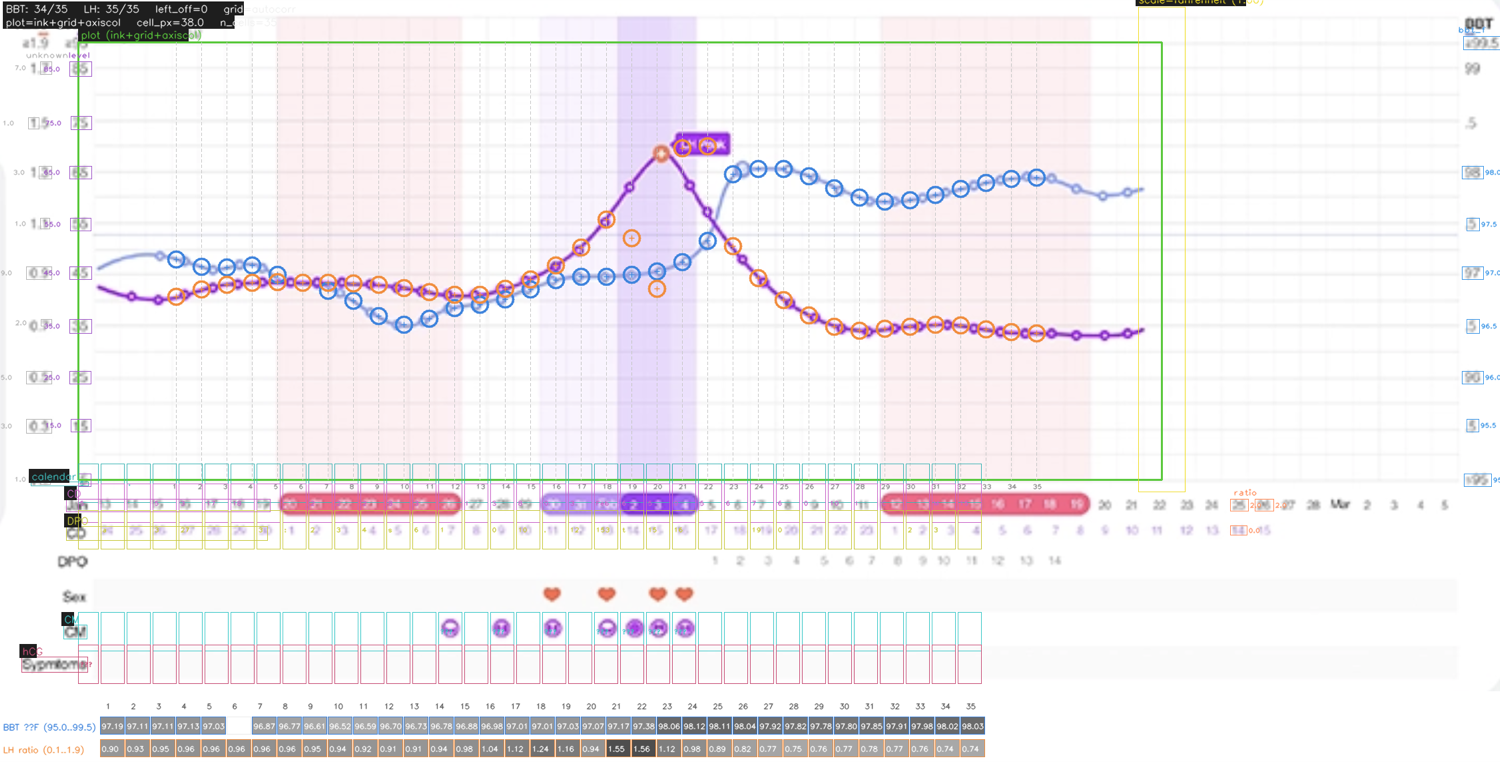
\includegraphics[width=\textwidth]{figures/overlays/overlay-3.png}
\caption{Overlay for \texttt{real-screen-3}, a dense $\approx\!42$-day chart whose
LH signal is the \emph{purple} ``Level'' line. Here the detector switches from
discrete markers to per-cell line sampling: the densely-packed blue and orange
rings track the continuous curves cell by cell, the chart is left-packed into the
35-day window and flagged \texttt{truncated}, and the purple Level line is
correctly chosen as the LH source over the orange Ratio line.}
\label{fig:overlay3}
\end{figure}

\subsection{The browser port}
\label{sec:cv-browser}
The production tool runs the pipeline entirely in the browser. The only two
OpenCV primitives that are not pure arithmetic, connected-component
labeling and morphological dilation, are reimplemented in pure TypeScript
(an eight-connectivity flood-fill with bounding-box and centroid
statistics, and a separable rectangular structuring element). As a result,
\textbf{no OpenCV.js or WASM build of OpenCV is required}; the only model
asset is the PaddleOCR ONNX, which is executed by ONNX Runtime Web exactly
like the forest models (Section~\ref{sec:ondevice}). The TypeScript port
emits a \code{ChartResultCv} type that mirrors the Python \code{ChartResult}
field for field, and is parity-tested against the Python reference.

\subsection{A neural alternative we explored but did not ship}
\label{sec:cnn-alt}
For completeness we record the convolutional network we built and evaluated
before settling on the classical pipeline. It is a compact, fully
convolutional encoder in the MobileNet family
\cite{howard2017mobilenets,sandler2018mobilenetv2}: a strided stem and six
depthwise-separable blocks downsampling only to $/8$, feeding three decode
heads (Figure~\ref{fig:visionarch}). Its distinctive element is a
per-series \emph{soft-argmax over height}~\cite{nibali2018numerical}. A
$1\times1$ convolution produces one heatmap channel per series, a softmax
over the height dimension yields a vertical probability distribution, and
the expected vertical coordinate \emph{is} the predicted value,
\begin{equation}
\bm{p} = \softmax_{h}\!\left(\text{heat}/\tau\right),\qquad
\text{value}_{s,w} = \sum_{i=1}^{h} p_{s,i,w}\, y_i \in [0,1],
\end{equation}
which makes ``value $=$ vertical position'' true by construction. A presence head
(height-pooled) and a unit-classification head complete the network. Trained on
procedurally rendered charts via a two-stage sim-to-real curriculum (generic
pre-training, then a Premom-specific fine-tune) with a masked-Huber $+$ BCE $+$
cross-entropy loss, the v2 network (\num{4.13}M parameters, \SI{16.6}{\mega\byte}
ONNX) reached a present-day value MAE of \num{0.022} of the axis span and a
presence $F_1$ of \num{0.934} on synthetic validation.

Despite these respectable numbers, we did \emph{not} deploy it, for the reasons
in Section~\ref{sec:why-cv}: it offers no auditability, produces no calendar
table, and carries a sim-to-real risk that the classical pipeline avoids by
construction. We include its architecture here only as a documented baseline.

\begin{figure}[H]
\centering
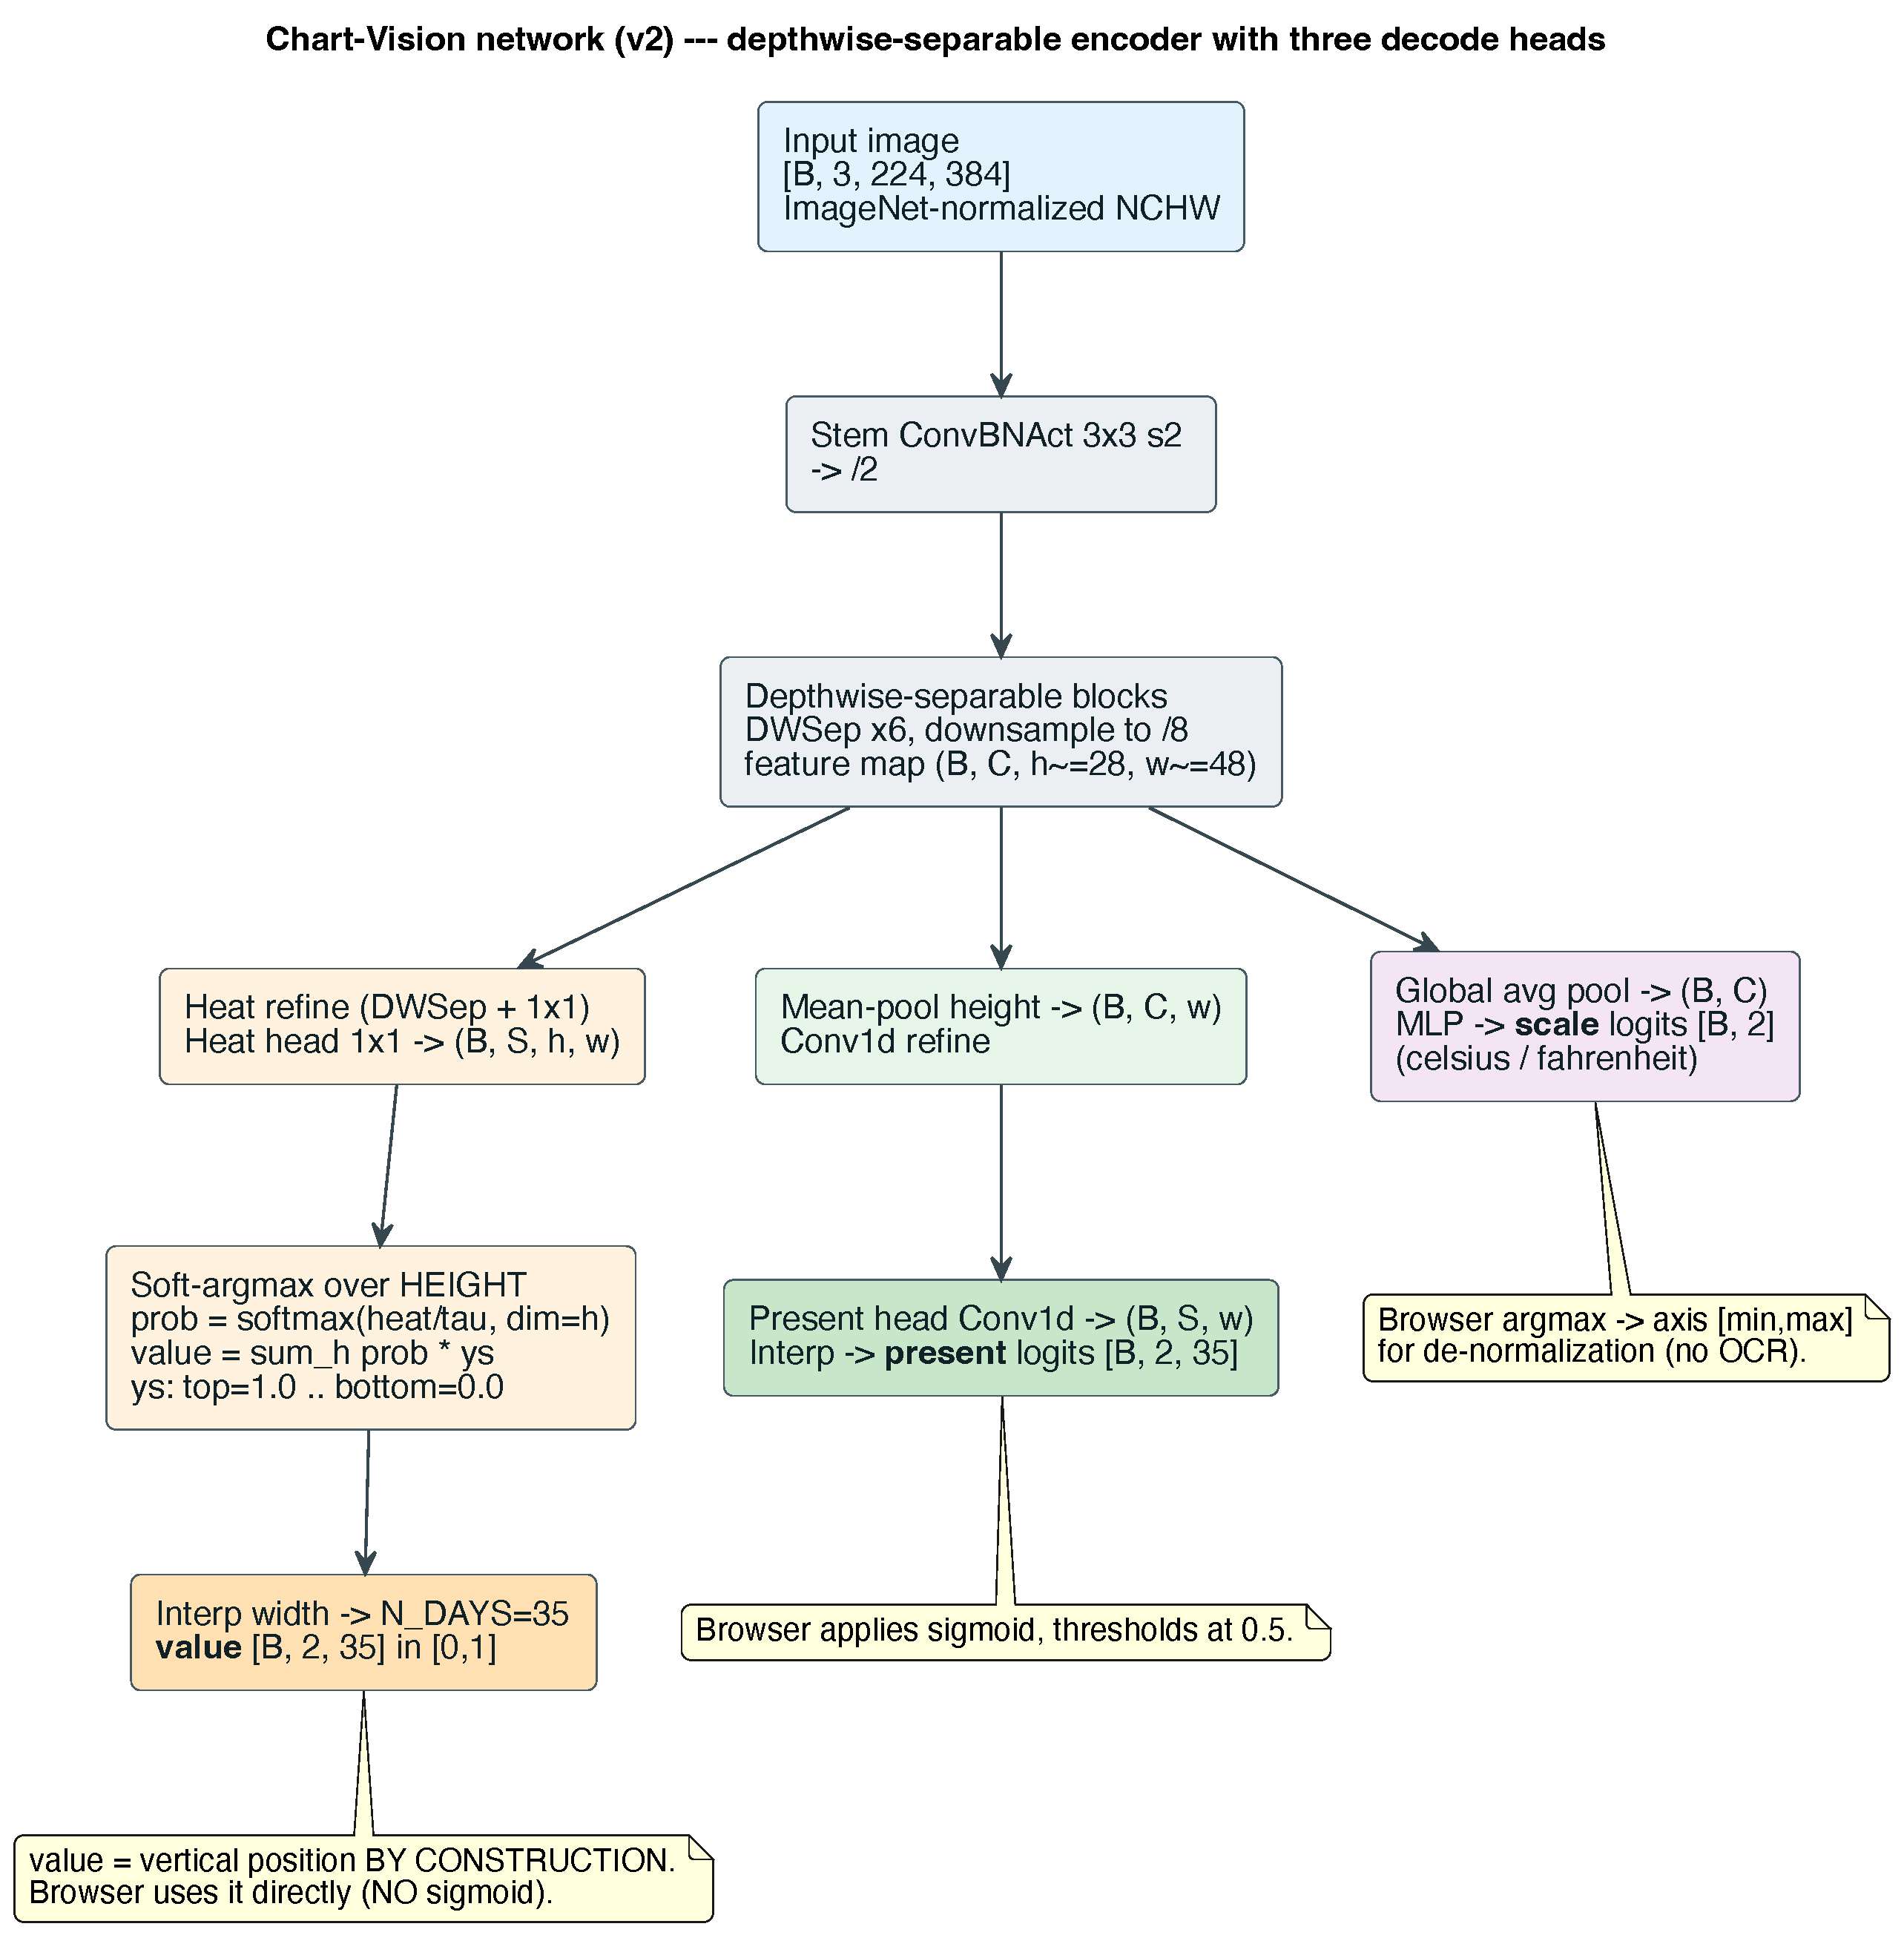
\includegraphics[width=0.95\textwidth]{figures/vision-architecture.pdf}
\caption{The \emph{unshipped} neural baseline: a depthwise-separable encoder
feeding a soft-argmax value head, a presence head, and a unit-classification
head. Retained for reference; the deployed vision stage is the classical pipeline
of Figure~\ref{fig:cvpipeline}.}
\label{fig:visionarch}
\end{figure}

\subsection{A hybrid digitization router}
The classical pipeline is the default of three on-device routes for reading a
screenshot (Figure~\ref{fig:import}). The deterministic CV pipeline runs first;
the manual column-scan calibrator gives the user a fully transparent fallback;
and the neural baseline of Section~\ref{sec:cnn-alt} remains available as an
experimental option. All routes converge on the same per-day series structure and
feed the forest classifier.

\begin{figure}[H]
\centering
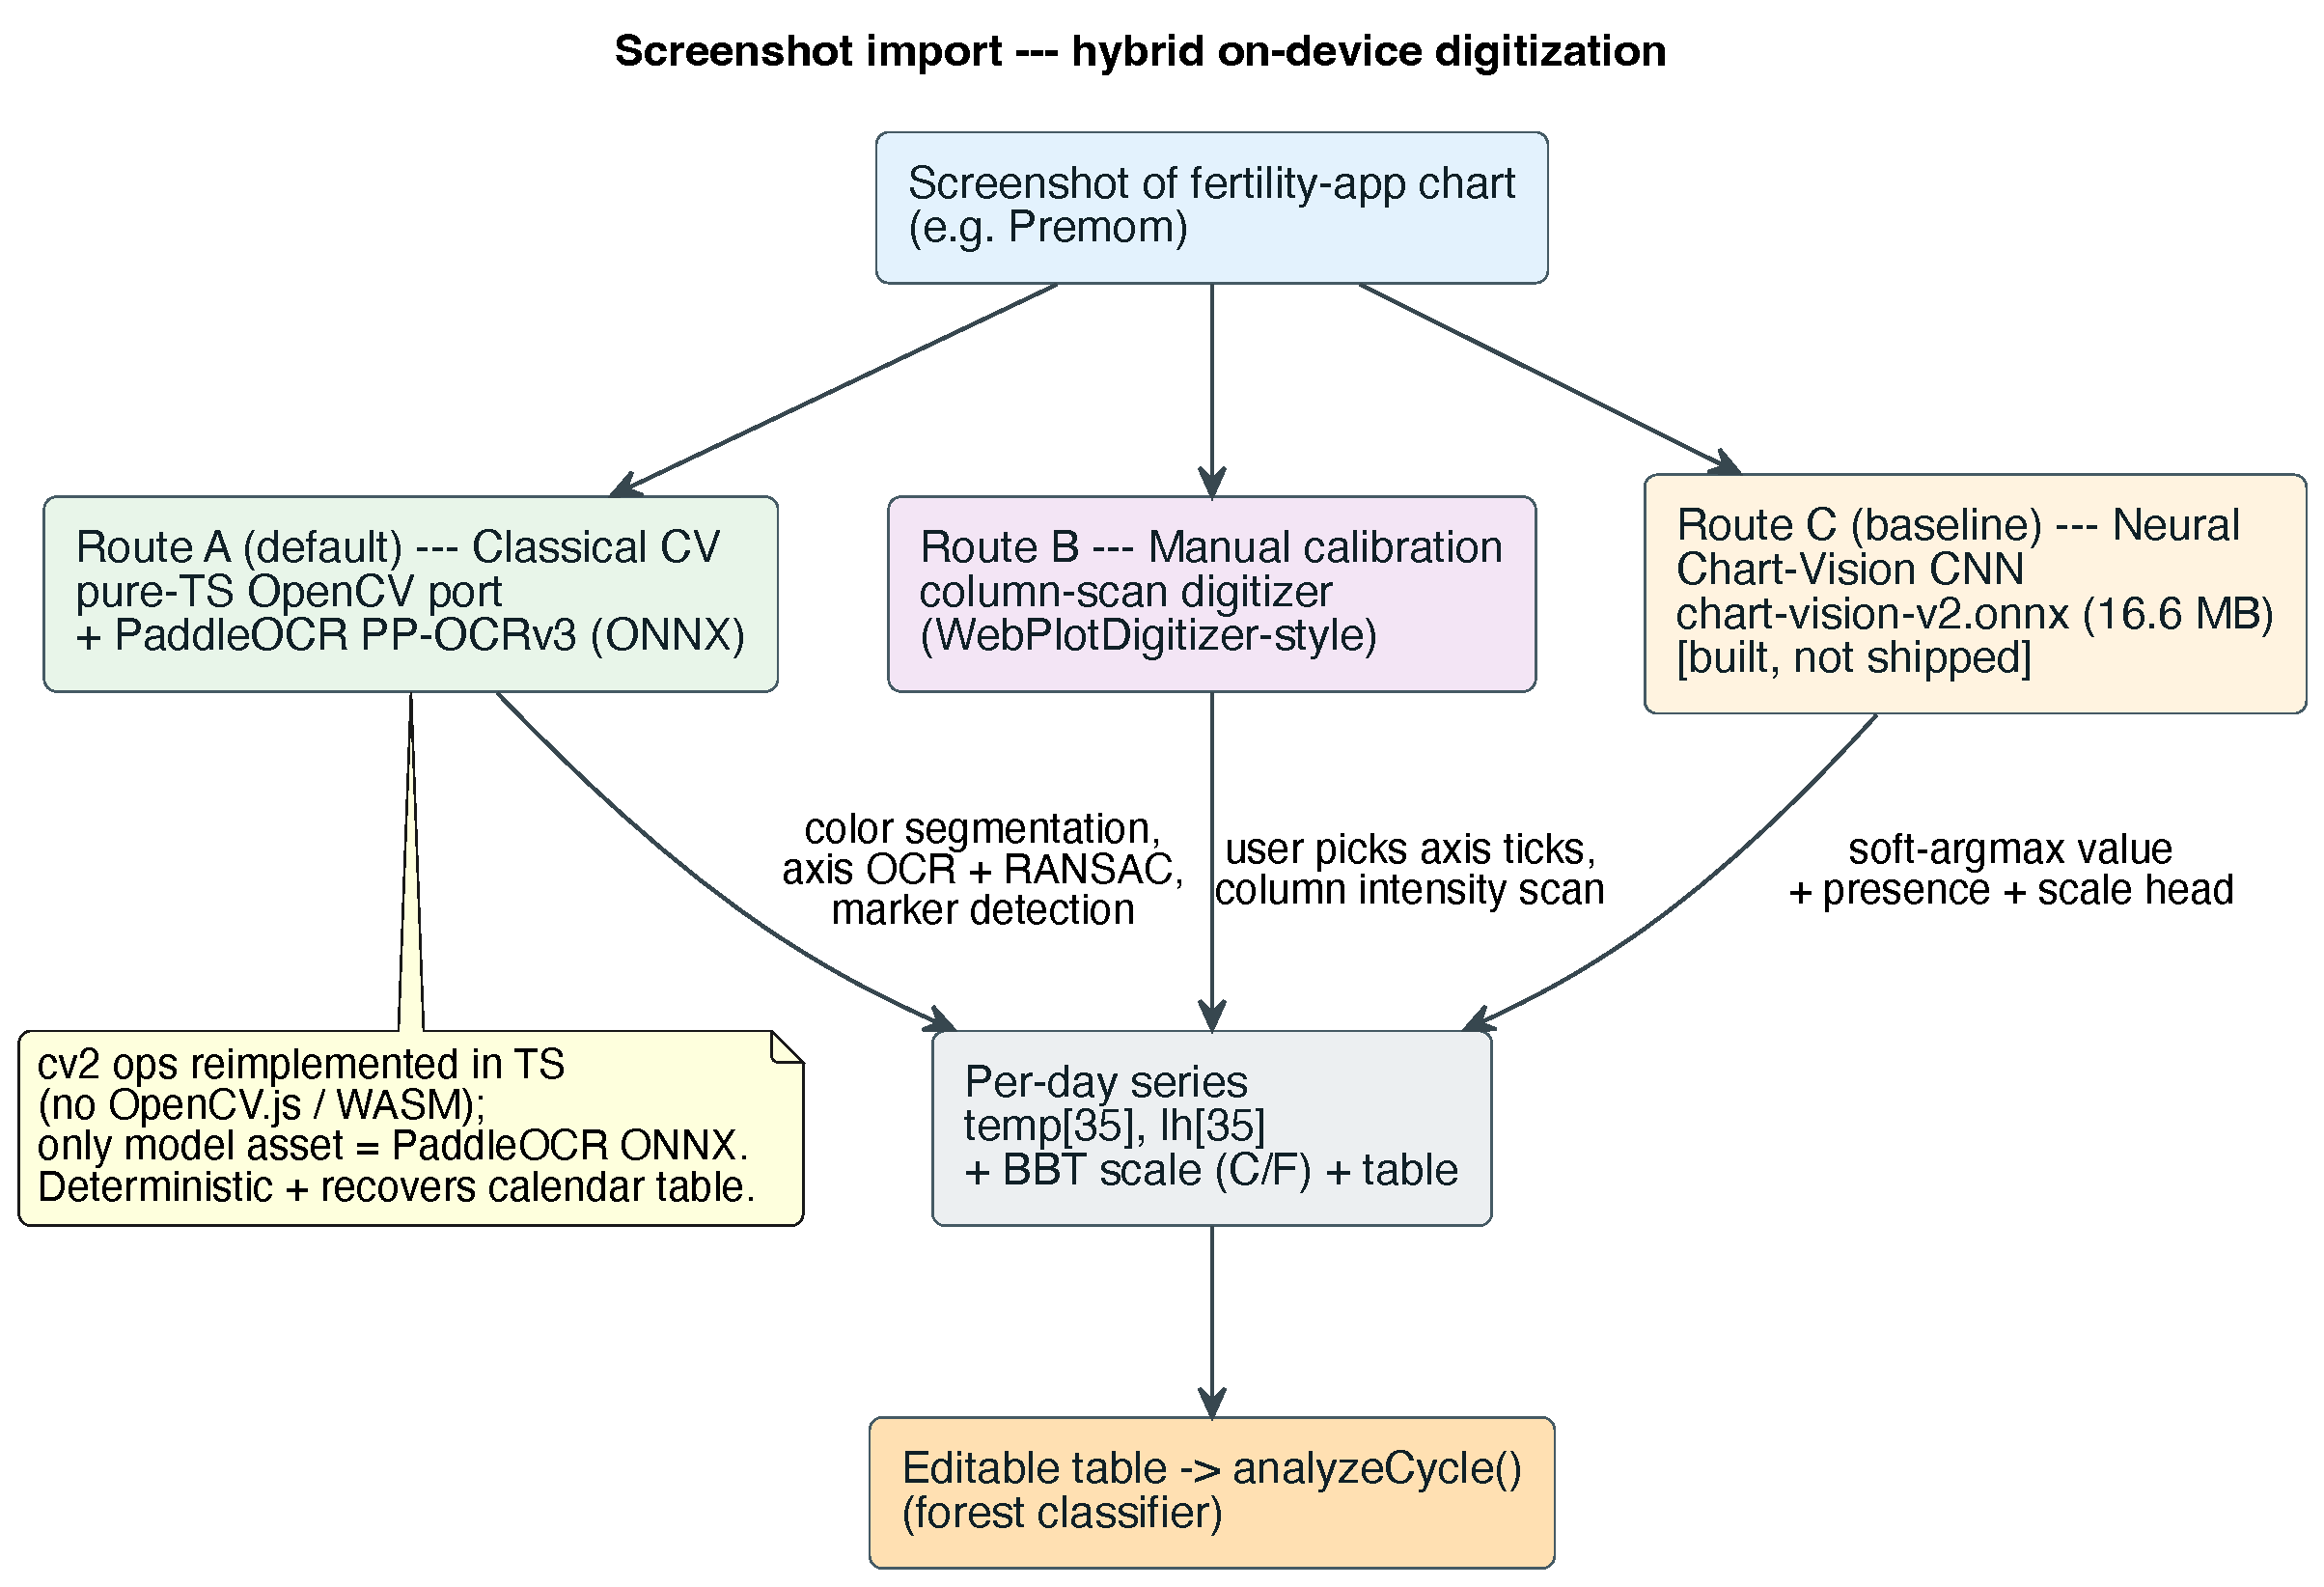
\includegraphics[width=0.96\textwidth]{figures/screenshot-import.pdf}
\caption{Hybrid on-device digitization. The deployed default is the deterministic
classical-CV pipeline ($+$ PaddleOCR); a manual calibrator and the neural baseline
are alternative routes. All produce the same structured series consumed by the
forest classifier.}
\label{fig:import}
\end{figure}

%==============================================================================
\section{Shipping models on-device}
\label{sec:ondevice}
%==============================================================================

\subsection{ONNX as the lingua franca}
Every model (the forest, the isolation forest, the vision network, and the
OCR) is exported to ONNX~\cite{onnx2017} and executed by ONNX Runtime Web on
the WebAssembly backend~\cite{onnxruntimeweb}. ONNX decouples the training
framework (scikit-learn, PyTorch) from the deployment runtime and provides
a single, auditable artifact whose operator set can be pinned to exactly
what the browser runtime supports.

\subsection{From artifact to asset}
Exported \code{.onnx} files and their JSON manifests are written to the
\file{model/artifacts/} directory. A build step (\file{scripts/sync-assets.mjs})
copies them into the application's \file{public/models/} directory, from which
the Cloudflare Worker serves them as same-origin static assets. The WASM runtime
binary is emitted by the bundler with a content hash and served from the same
origin, so no cross-origin CDN is involved and no special isolation headers are
required.

\subsection{Versioned, checksum-validated caching}
The heavy ONNX files would be wasteful to re-download on every visit, so they are
cached in IndexedDB through Dexie. The cache is content-addressed and versioned:
each blob is keyed by \code{\${version}:\${fileName}} and validated against the
SHA-256 recorded in the manifest. On a version bump or a checksum mismatch the
stale entry is evicted and the file refetched; older versions of a file are
purged to bound storage. After the first successful load the application is fully
offline-capable.

\begin{lstlisting}[language=ts,caption={Checksum-keyed cache lookup and eviction
(from \file{modelCache.ts}).}]
const cached = await db().modelFiles.get(key);   // key = `${version}:${fileName}`
if (cached && cached.sha256 === sha256) return cached.data;   // hit
if (cached) await db().modelFiles.delete(key);                // stale -> evict
const data = await fetchWithProgress(url, fileName, expectedBytes, onProgress);
if (await sha256Hex(data) === sha256) {           // integrity gate
  await db().modelFiles.where("fileName").equals(fileName)
           .and(r => r.version !== version).delete();          // purge old versions
  await db().modelFiles.put({ key, version, fileName, sha256, data, ... });
}
\end{lstlisting}

\subsection{Inference lifecycle}
Figure~\ref{fig:seq} traces the full sequence for both a cold start (cache
miss) and a warm start (cache hit). On a cold start the runtime fetches the
manifest, streams the model with progress reporting, verifies the
checksum, persists it, and constructs an inference session. On a warm start
it loads directly from IndexedDB with no network access. Inference itself
(feature extraction, the classifier forward pass, the confidence gate of
Equation~\eqref{eq:gate}, and the OOD percentile) runs entirely in WASM.

\begin{figure}[H]
\centering
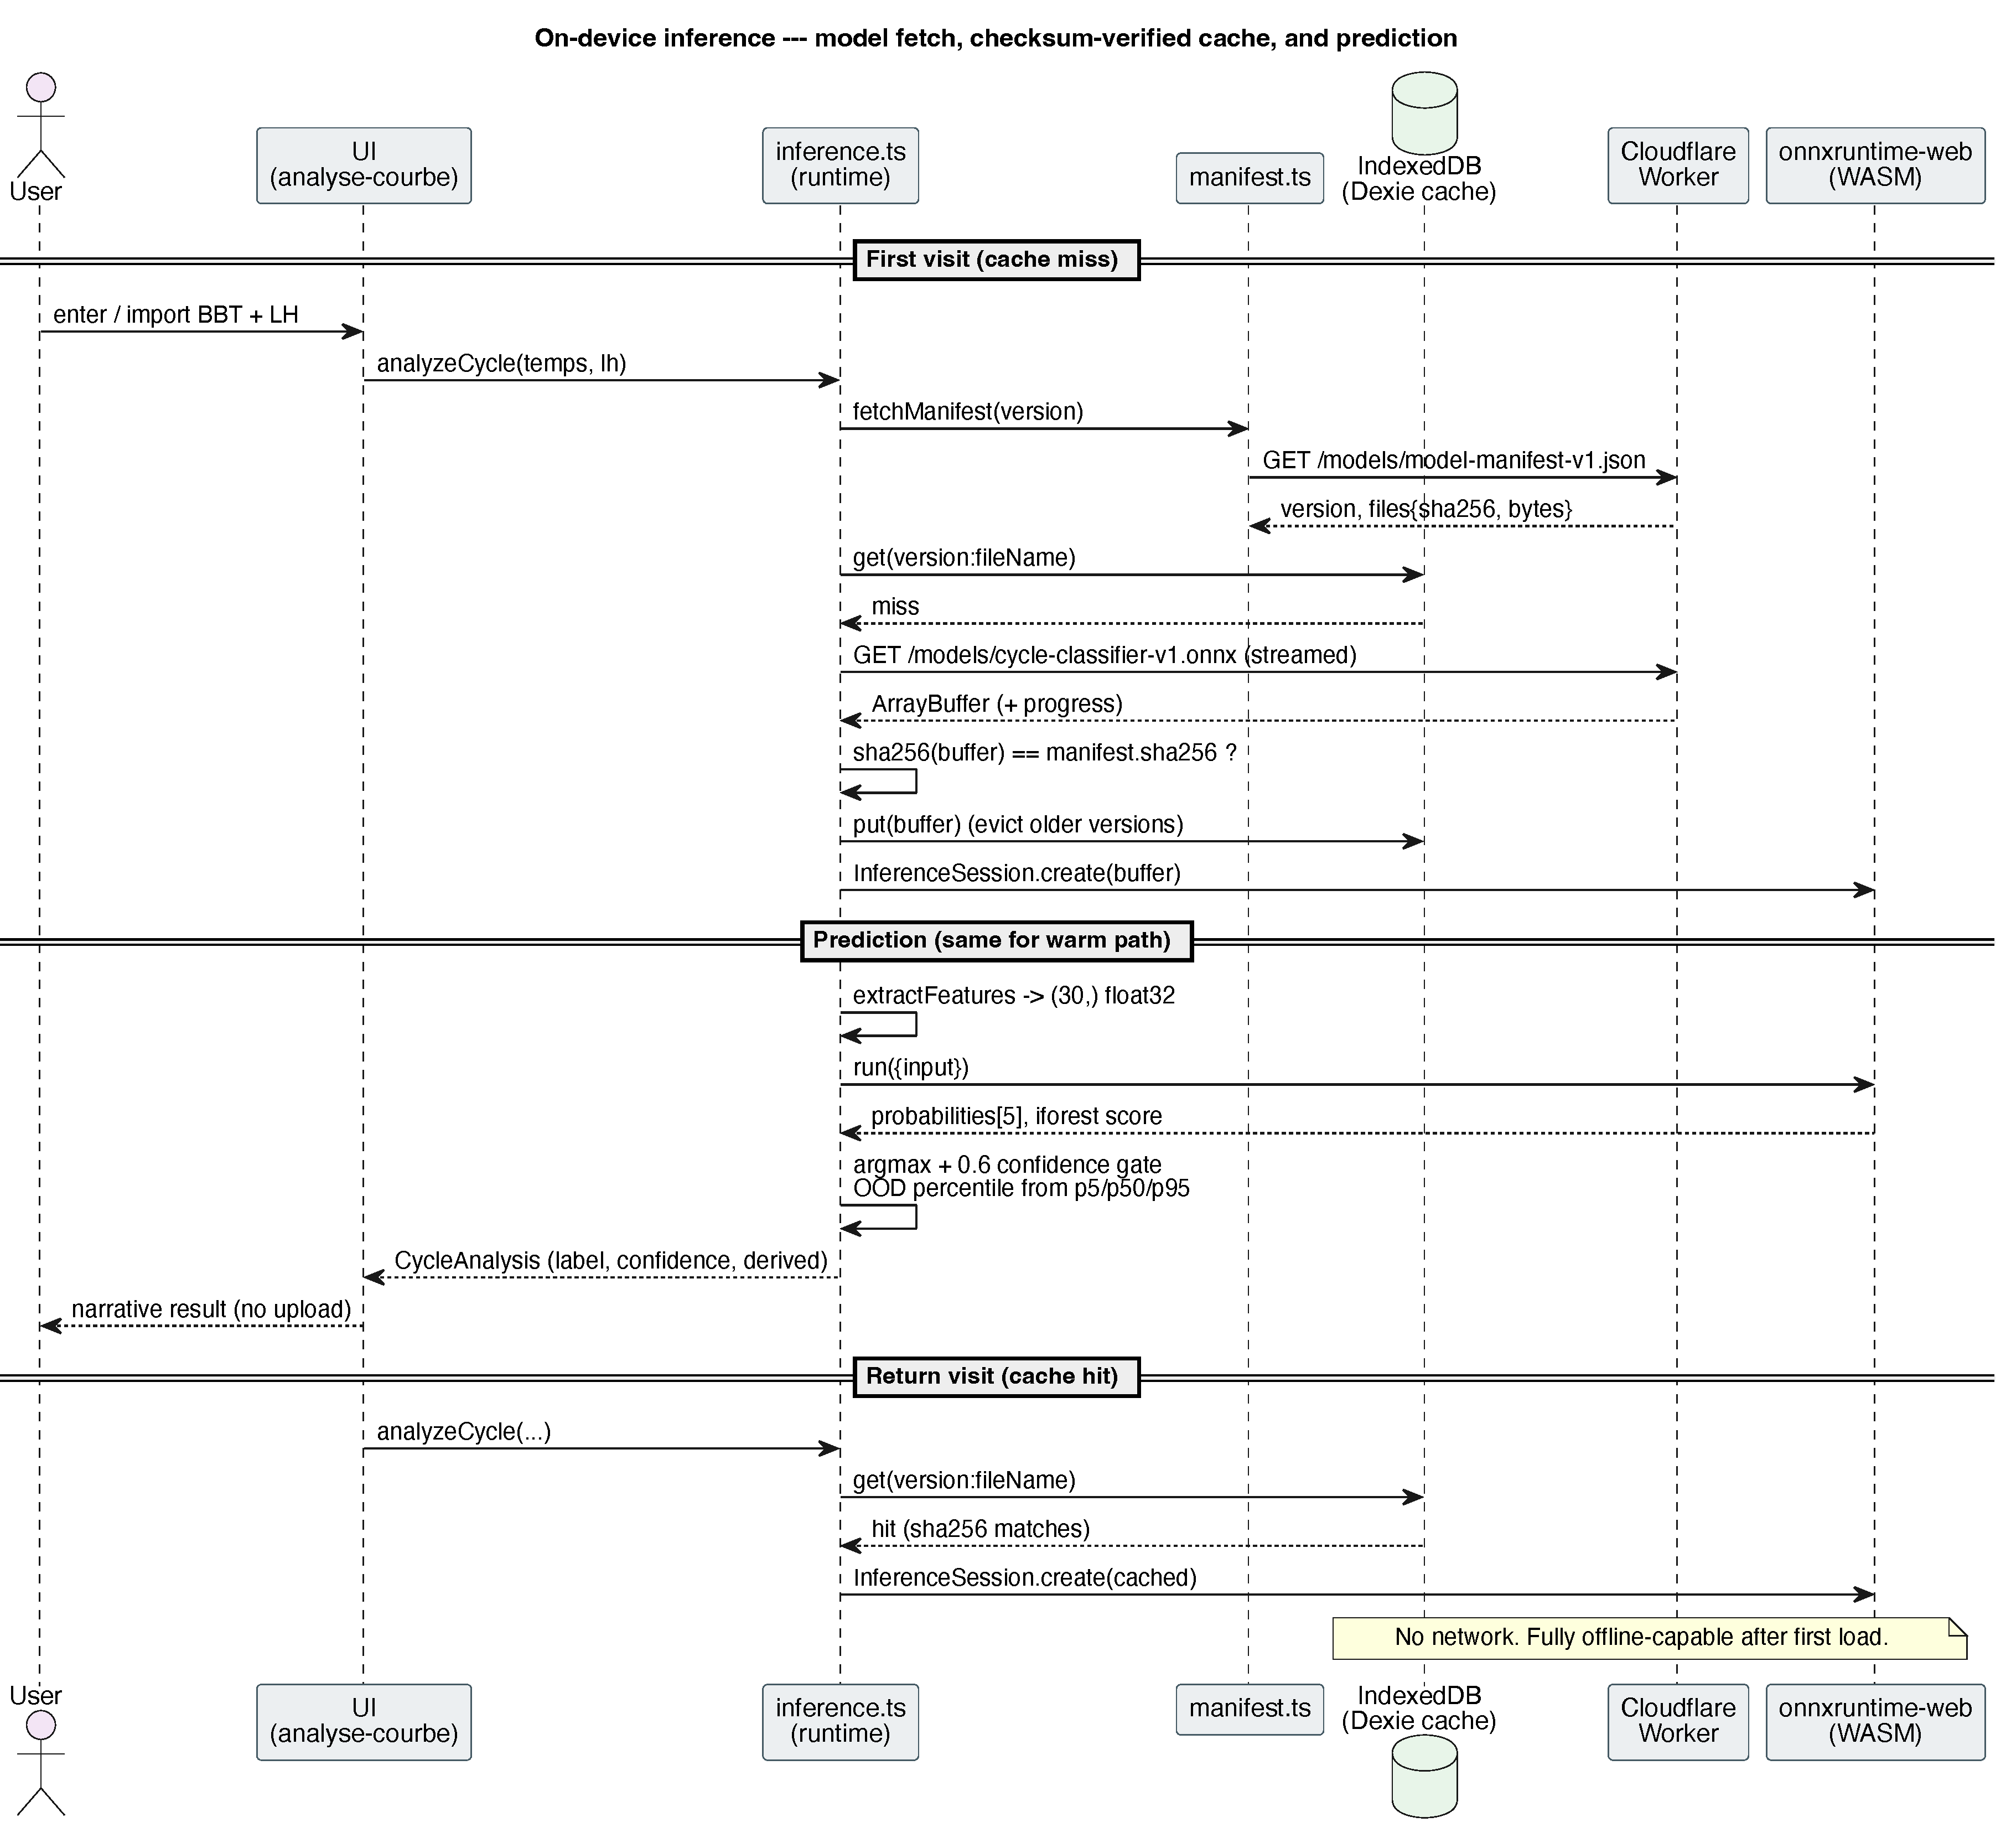
\includegraphics[width=\textwidth]{figures/ondevice-sequence.pdf}
\caption{On-device inference lifecycle. The cold path (cache miss) verifies a
checksum and persists the model; the warm path is network-free. No cycle datum
is ever transmitted.}
\label{fig:seq}
\end{figure}

\subsection{The parity contract}
Feature extraction is implemented twice: canonically in Python
(\file{features.py}) for training, and in TypeScript (\file{features.ts}) for
the browser. Any divergence would silently degrade accuracy, because the model
was trained on the Python features but evaluated on the TypeScript ones. We
therefore treat numerical parity as a hard contract enforced by a fixture-based
test: the Python implementation emits reference vectors that the TypeScript
implementation must reproduce exactly.

\begin{property}[Cross-language feature parity]
For every input pair $(\bm t, \bm\ell)$ in the fixture set,
$\phi_{\text{py}}(\bm t,\bm\ell) = \phi_{\text{ts}}(\bm t,\bm\ell)$ within
floating-point tolerance. The export likewise guarantees
$\big\lVert \Pr_{\text{sklearn}} - \Pr_{\text{onnx}} \big\rVert_\infty < 10^{-3}$
for the classifier. The vision pipeline likewise carries a
Python$\leftrightarrow$TypeScript parity contract: the browser port reproduces
the reference \code{ChartResult} of the Python implementation field for field,
verified by fixtures.
\end{property}

%==============================================================================
\section{Privacy and threat model}
%==============================================================================

The system's privacy posture follows directly from its architecture rather
than from policy promises. There is no account and no server-side data
store; the only egress is the one-time download of public model files.
Consequently:
\begin{itemize}
  \item \textbf{Confidentiality at rest and in transit.} Cycle data exist only in
  the page's memory and (optionally) the user's own local storage; they are never
  serialized to a network request.
  \item \textbf{No linkage.} Without an account or tracking identifier, analyses
  cannot be associated with an individual across sessions or devices.
  \item \textbf{Integrity of models.} The SHA-256 gate ensures that a tampered or
  corrupted model file is rejected rather than executed, providing a basic
  supply-chain integrity check for the cached artifacts.
  \item \textbf{Regulatory alignment.} By never processing personal data on the
  server, the design sidesteps the bulk of the obligations that GDPR
  \cite{gdpr2016} attaches to special-category data.
\end{itemize}
The residual trust assumption is the integrity of the delivered application
code and WASM runtime, which is identical to that of any web page, and
which subresource integrity and the same-origin policy mitigate.

%==============================================================================
\section{Discussion and limitations}
%==============================================================================

\paragraph{Determinism over learned perception.} The deployed vision stage
is a deterministic pipeline of hand-tuned stages rather than a learned
model. Its main risk is therefore brittleness to chart idioms it was not
tuned for: a new app's color palette, axis layout, or marker style may
require new HSV bands or axis profiles. We accept this in exchange for
auditability, a structured calendar-table side-output, and the absence of
any sim-to-real gap. The neural baseline of Section~\ref{sec:cnn-alt},
trained with domain randomization and a Premom-specific fine-tune, remains
available should a learned route ever be preferred. Broadening either
approach to more app idioms is the natural next step.

\paragraph{Synthetic-only training of the forest.} The forest is trained
without real labeled data. Its labels are by construction consistent with
the clinical rules, so the principal risk is distribution shift between
synthetic archetypes and real cycles. The isolation-forest backstop
mitigates this risk, but does not eliminate it.

\paragraph{Confusion between adjacent classes.} The largest classification errors
fall between clinically adjacent categories (confirmed vs.\ doubtful ovulation),
which reflects genuine ambiguity rather than model failure. The calibrated
probabilities and the confidence gate of Equation~\eqref{eq:gate} convert this
ambiguity into an explicit, user-visible uncertainty rather than a falsely
confident label.

\paragraph{Client compute budget.} A single-thread WASM runtime keeps deployment
simple but caps throughput. The geometric vision pipeline and the modest forest
are both chosen to stay within an interactive latency budget on commodity
devices; multi-threaded WASM or WebGPU execution providers are a forward-looking
optimization.

%==============================================================================
\section{Conclusion}
%==============================================================================

FertiLuna shows that a non-trivial machine-learning product, pairing a
deterministic computer-vision perception stage with a calibrated tabular
reasoning model, can be delivered \emph{entirely} on-device in the web
browser without compromising analytical quality. The two-stage
decomposition aligns each task with an appropriate inductive bias: a
transparent, auditable geometric pipeline reads the chart (and recovers
its calendar table as a side-output), while a synthetic-trained,
probability-calibrated forest renders the clinical judgment. Choosing
classical computer vision over a learned model for perception trades a
little engineering effort for determinism, a richer structured output,
and the elimination of any sim-to-real gap. We argue this is the right
trade for a privacy-first health tool. The ONNX-plus-IndexedDB shipping
pipeline turns the remaining model assets into versioned,
integrity-checked, offline-capable assets, and the enforced cross-language
parity contract closes the loop between the Python reference and the
browser runtime. Together, these choices yield a system whose privacy
guarantees are structural, not merely contractual.

%==============================================================================
\printbibliography[heading=bibnumbered,title={References}]
%==============================================================================

\end{document}
